\section{Theoretische Grundlagen}

Um die kürzeste Route zwischen zwei Orten in einem Straßennetz zu ermitteln, kann man die
Graphentheorie als Teilgebiet der Mathematik heranziehen.

\subsection{Graphentheorie}

Ein Graph ist eine abstrakte Struktur, die Objekte und deren Verbindungen untereinander modellieren kann.
Die in der Graphentheorie verwendeten Termini belaufen sich dabei auf Ecken (engl: \textit{nodes} oder \textit{vertices}) für Objekte und Kanten (engl: \textit{edges}) für Verbindungen.
(\cite[49]{kurt})

Ein Vorteil von Graphen ist deren einfache Struktur.
Dabei werden die Ecken als Punkte und die Kanten als Linien oder Pfeile dargestellt (Abb.~\ref{fig:simple}) (\cite[49]{kurt}).

Mathematisch ausgedrückt ist ein Graph ~$G$ die Funktion aus einer endlichen Eckenmenge ~$V$ und einer endlichen Kantenmenge ~$E$ (\cite[4]{theory})

	$$G = (V,E)$$

Für den Graphen in Abbildung ~\ref{simpleGraph} sehen ~$V$ und ~$E$ folgendermaßen aus:

$$V = \{(v_{1},v_{2},v_{3},v_{4},v_{5})\} $$
$$E = \{(v_{1}v_{2},v_{1}v_{3},v_{2}v_{3},v_{2}v_{3},v_{3}v_{5})\} $$

\begin{figure}[htb]
\centering
\begin{subfigure}{0.49\textwidth}
\centering
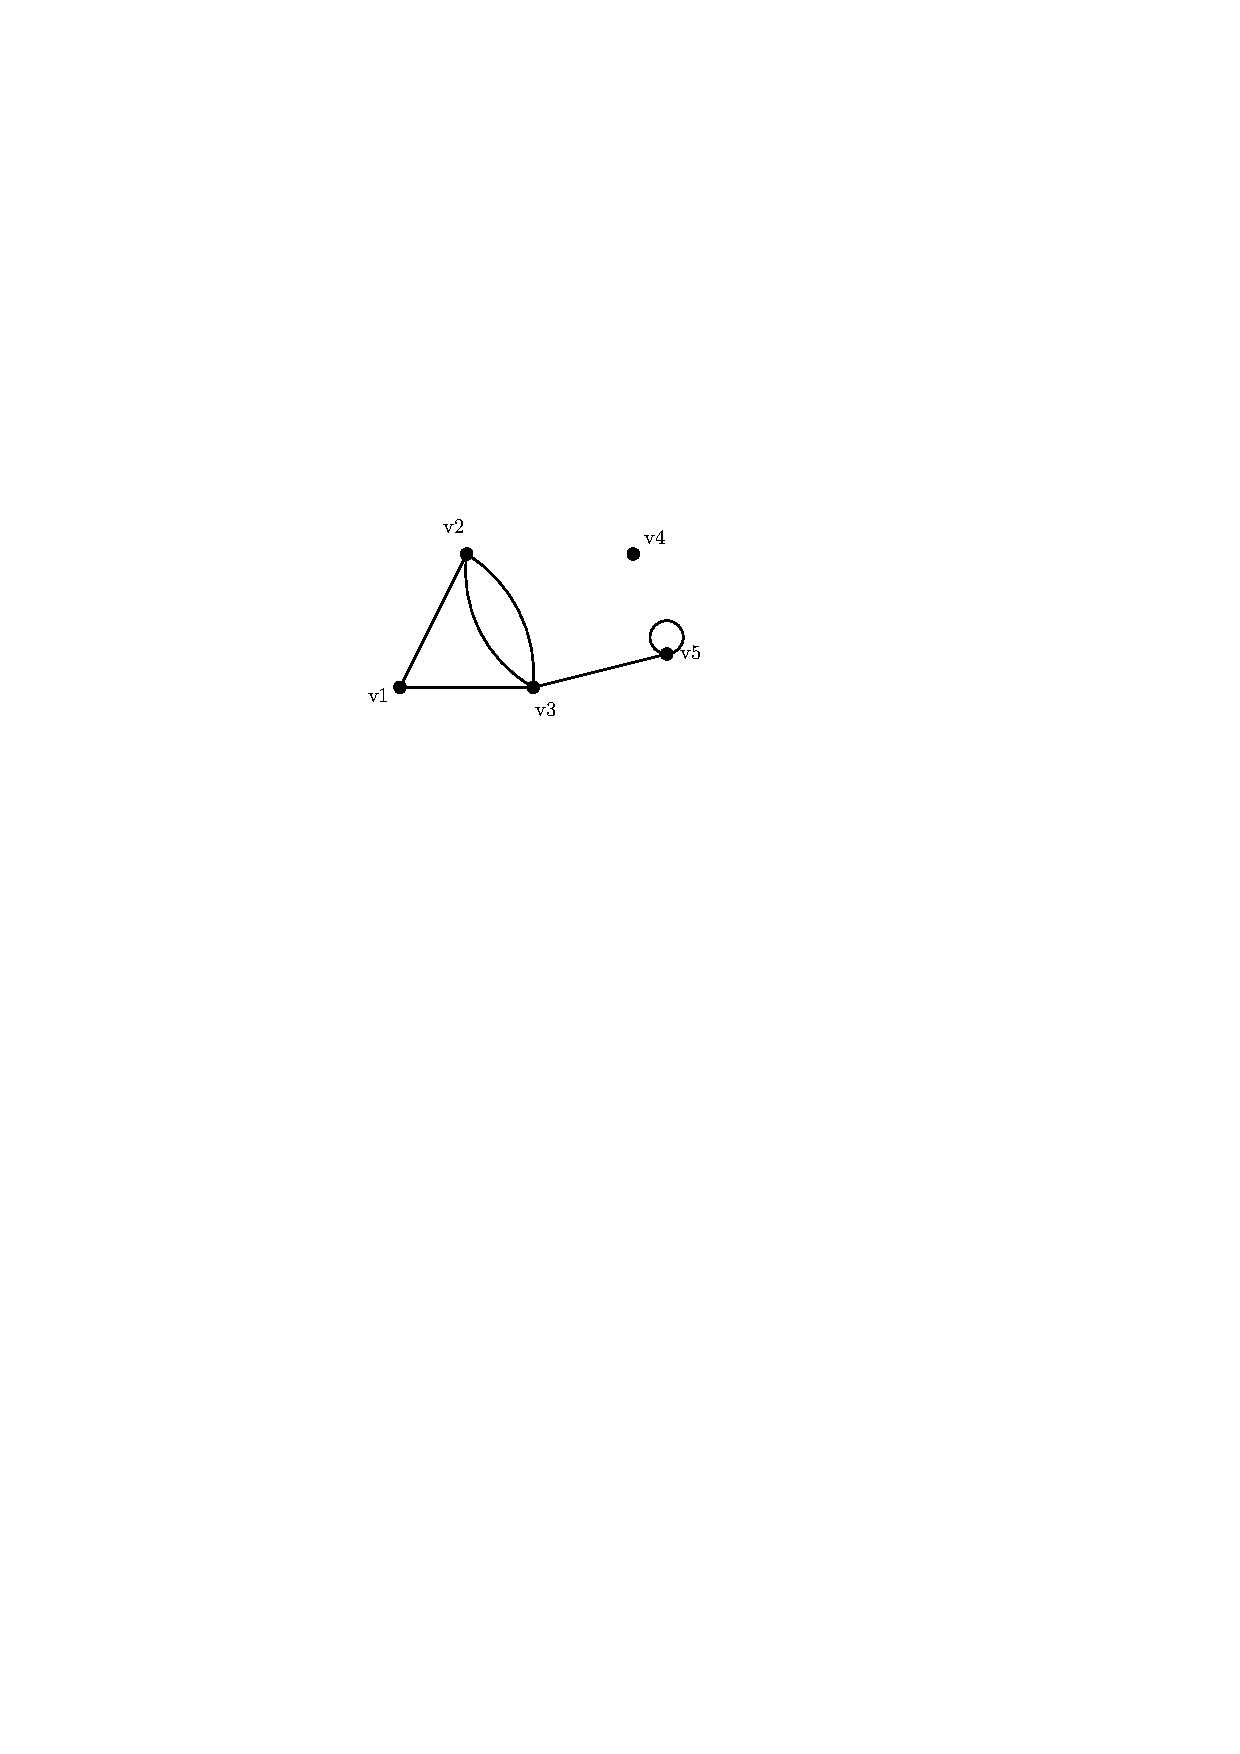
\includegraphics[width = \textwidth]{../media/simpel.pdf} \\
\caption{G}
\label{fig:simple}
\end{subfigure}
\begin{subfigure}{0.49\textwidth}
\centering
{
\begin{blockarray}{cccccc}
  & $v_{1}$ & $v_{2}$ & $v_{3}$ & $v_{4}$ & $v_{5}$ \\
\begin{block}{c(ccccc)}
  $v_{1}$ & 0 & 1 & 1 & 0 & 0 \\
  $v_{2}$ & 1 & 0 & 2 & 0 & 0 \\
  $v_{3}$ & 1 & 2 & 0 & 0 & 1 \\
  $v_{4}$ & 0 & 0 & 0 & 0 & 0 \\
  $v_{5}$ & 0 & 0 & 1 & 0 & 1 \\
\end{block}
\end{blockarray}
}
\vspace{0.1cm}
\caption{Adjazenzmatrix von G}
\label{mx:simple}
\end{subfigure}
\caption{Ein simpler Graph G und seine Adjazenzmatrix}
\label{simpleGraph}
\end{figure}

Zwischen zwei Ecken können einfache, mehrfache oder keine Kanten bestehen.
Darüber hinaus können sie mit sich selbst verbunden sein und eine sogenannte Schlinge bilden (Abb.~\ref{fig:simple}).
Sind zwei Ecken durch eine Kante verbunden, werden sie als \textit{adjazent}(benachbart) bezeichnet.
Ist eine Ecke der Start- oder Endpunkt einer Kante, werden beide Objekte als \textit{inzident} zueinander bezeichnet.
Ist eine Ecke zu keiner Kante inzident, heißt sie \textit{isoliert}.
Ein Graph der keine isolierten Ecken besitzt heißt \textit{zusammenhängend}.(\cite[4\psq]{theory}) \par

Computer können Graphen verarbeiten, da sich alle Ecken und Kanten in Form von Matrizen speichern lassen.
Die Abbildung ~\ref{mx:simple} zeigt die Adjazenzmatrix des Graphen aus ~\ref{fig:simple}.
In einer Adjazenzmatrix werden die Nachbarschaften für die jeweilige Eckenkombination gespeichert.
Die Reihen stellen die Start- und die Spalten die Endecken dar.
Eine bestehende Kante wird mit einer ~$1$ dargestellt.
Wenn keine Verbindung besteht, wird dies durch die ~$0$ angezeigt.
Bestehen mehrere Kanten zwischen zwei Ecken, wird dies durch die Anzahl der bestehenden Kanten dargestellt (z.B. durch die Zahl $2$ für die Ecken $v_{2}$ und $v_{3}$).
Für ungerichtete Graphen ist eine Kante von $v_{1}$ nach $v_{2}$ äquivalent mit einer Kante von $v_{2}$ nach $v_{1}$.
Daher ist die Adjazenzmatrix für ungerichtete Graphen spiegelsymmetrisch entlang der Hauptdiagonale ($v_{1}v_{1} \rightarrow v_{5}v_{5}$).
Der Speicherbedarf für solch eine Matrix wird folglich halbiert, da eine Hälfte mithilfe der Anderen rekonstruiert werden kann (Abb.~\ref{mx:iso}).
Besitzt der Graph keine Schlingen, besteht die Hauptdiagonale lediglich aus Nullen und kann ebenfalls eingespart werden (\cite[19]{algorithms}).

Im Folgenden werden nur zusammenhängende Graphen ohne Schlingen betrachtet, da diese für viele Problemstellungen irrelevant sind (\cite[4\psq]{theory}).

\begin{figure}[htb]
\centering
\begin{subfigure}{0.42\textwidth}
\centering
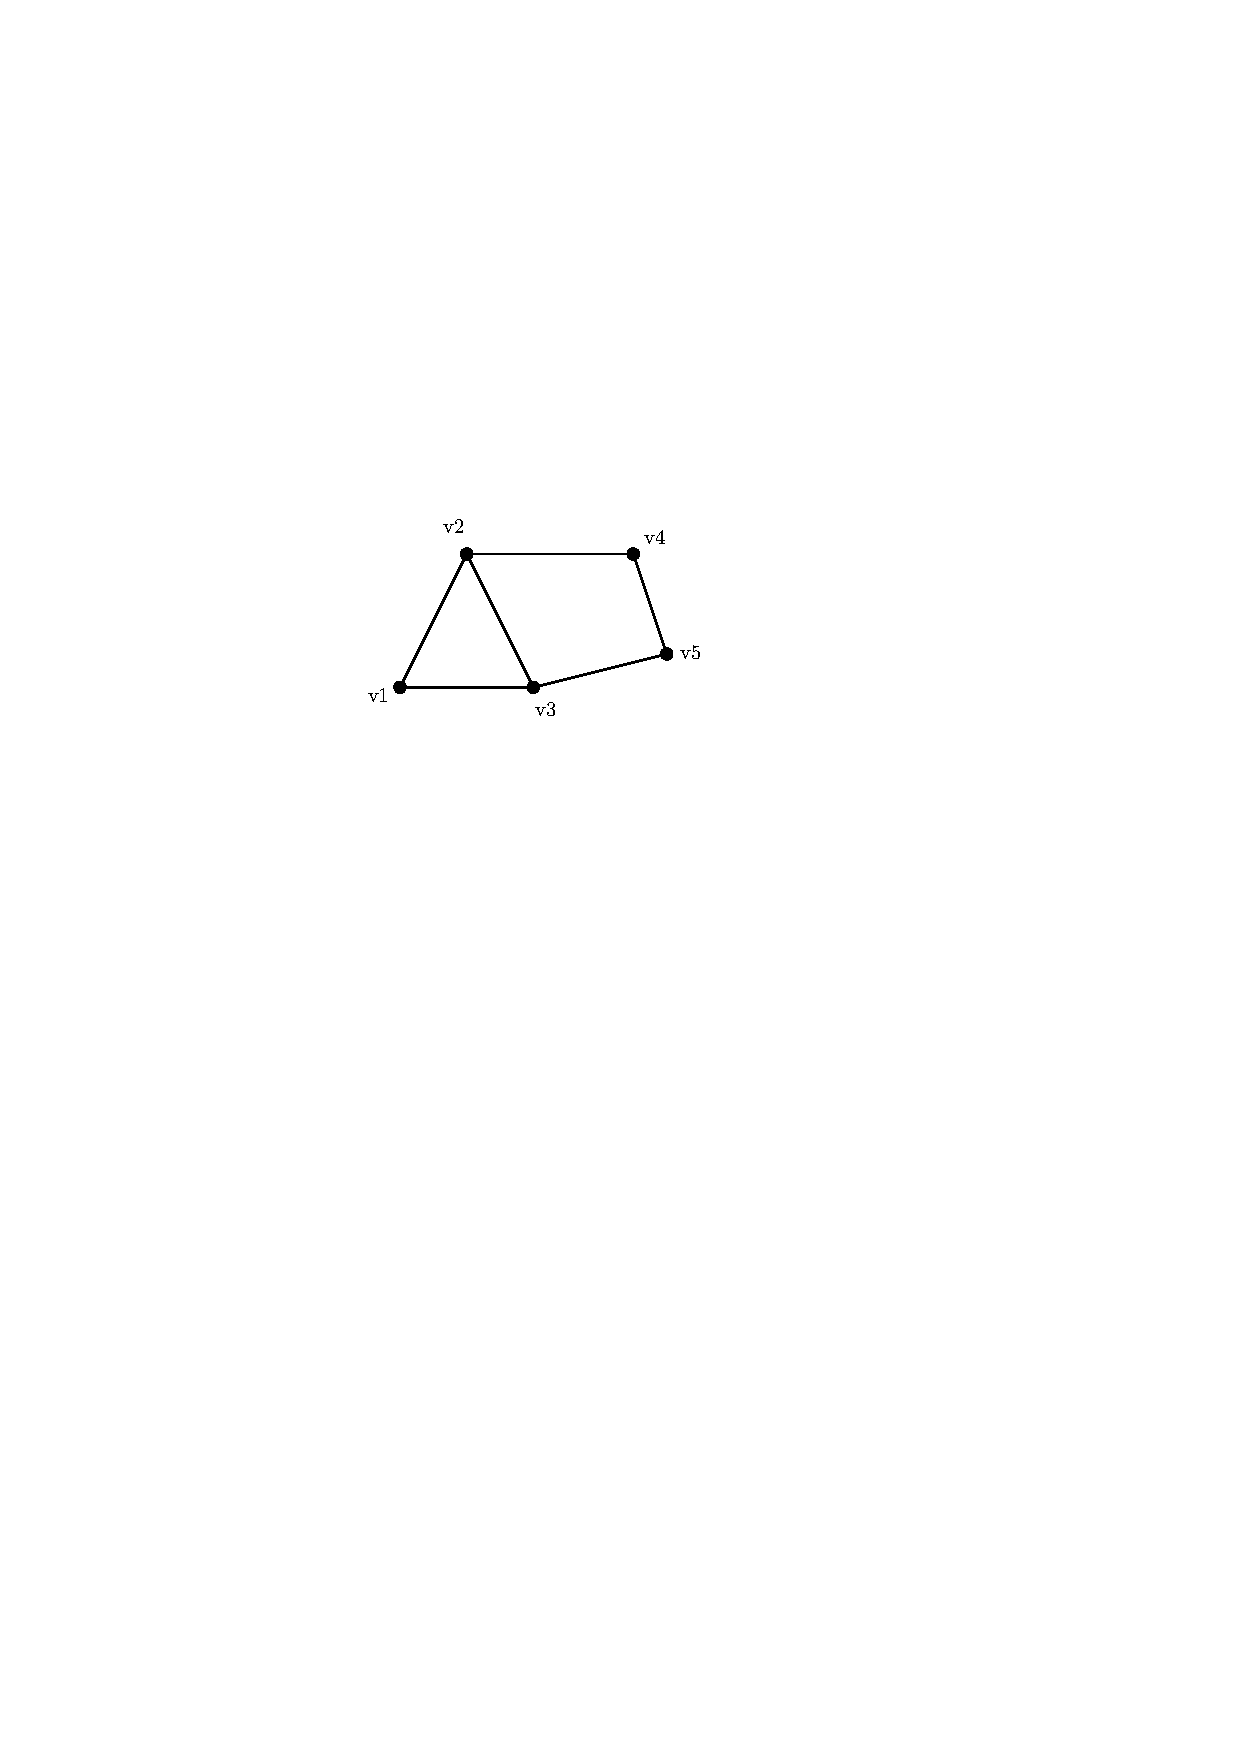
\includegraphics[width = \textwidth]{../media/iso1.pdf} \\
\caption{G}
\label{fig:iso1}
\end{subfigure}
\hspace{2cm}
\begin{subfigure}{0.30\textwidth}
\centering
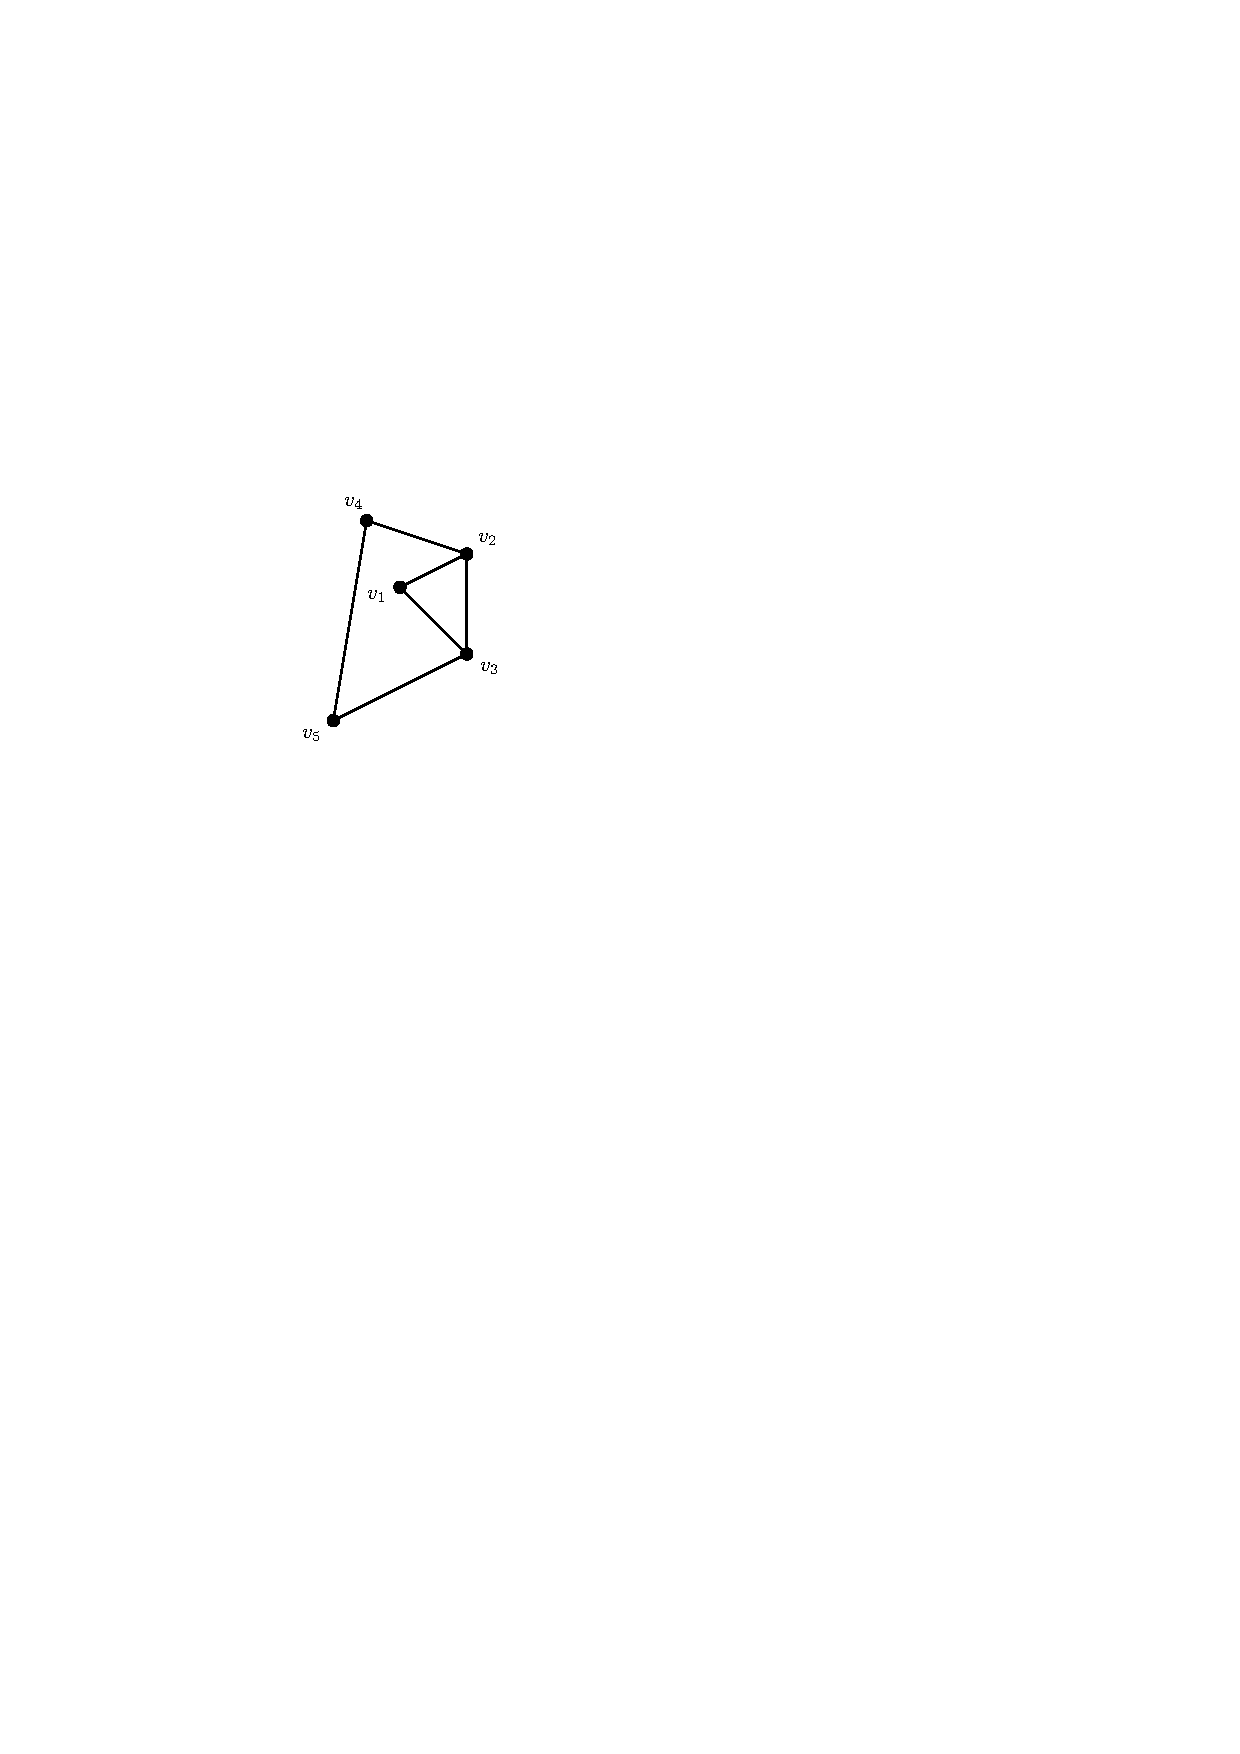
\includegraphics[width = \textwidth]{../media/iso2.pdf} \\
\caption{H}
\label{fig:iso2}
\end{subfigure}
\begin{subfigure}{0.40\textwidth}
\centering
\vspace{0.5cm}
{
\begin{blockarray}{cccccc}
  & $v_{1}$ & $v_{2}$ & $v_{3}$ & $v_{4}$ & $v_{5}$ \\
\begin{block}{c(ccccc)}
  $v_{1}$ & $\ddots$ & 1 & 1 & 0 & 0 \\
  $v_{2}$ &   & $\ddots$ & 1 & 1 & 0 \\
  $v_{3}$ &   &   & $\ddots$ & 0 & 1 \\
  $v_{4}$ &   &   &   & $\ddots$ & 1 \\
  $v_{5}$ &   &   &   &   & $\ddots$ \\
\end{block}
\end{blockarray}
}
\caption{Adjazenzmatrix von G und H}
\label{mx:iso}
\end{subfigure}
\caption{Zwei isomorphe Graphen G und H und ihre Adjazenzmatrix}
\label{isoGraph}
\end{figure}

Wenn zwei Graphen bei gleichbleibenden Nachbarschaften der Ecken aufeinander abgebildet werden können, spricht man von isomorphen Graphen (\cite[106]{theory}).
Daraus ergibt sich für isomorphe Graphen auch immer eine gleiche Adjazenzmatrix (Abb.~\ref{isoGraph}).


\subsubsection{Gerichtete Graphen}
Im Gegensatz zu einem ungerichteten Graphen, können bei einem gerichteten Graphen Kanten lediglich in einer Richtung durchlaufen werden.
Die Kanten werden daher durch Pfeile, anstatt durch Linien, dargestellt.

$$G = (V,R)$$

Demnach muss in Abbildung~\ref{fig:directed}, um von der Ecke $v_{5}$ nach $v_{4}$ zu gelangen, der Weg über die Ecken $v_{3}$ und $v_{2}$ führen.

\begin{figure}[htb]
\centering
\begin{subfigure}{0.49\textwidth}
\centering
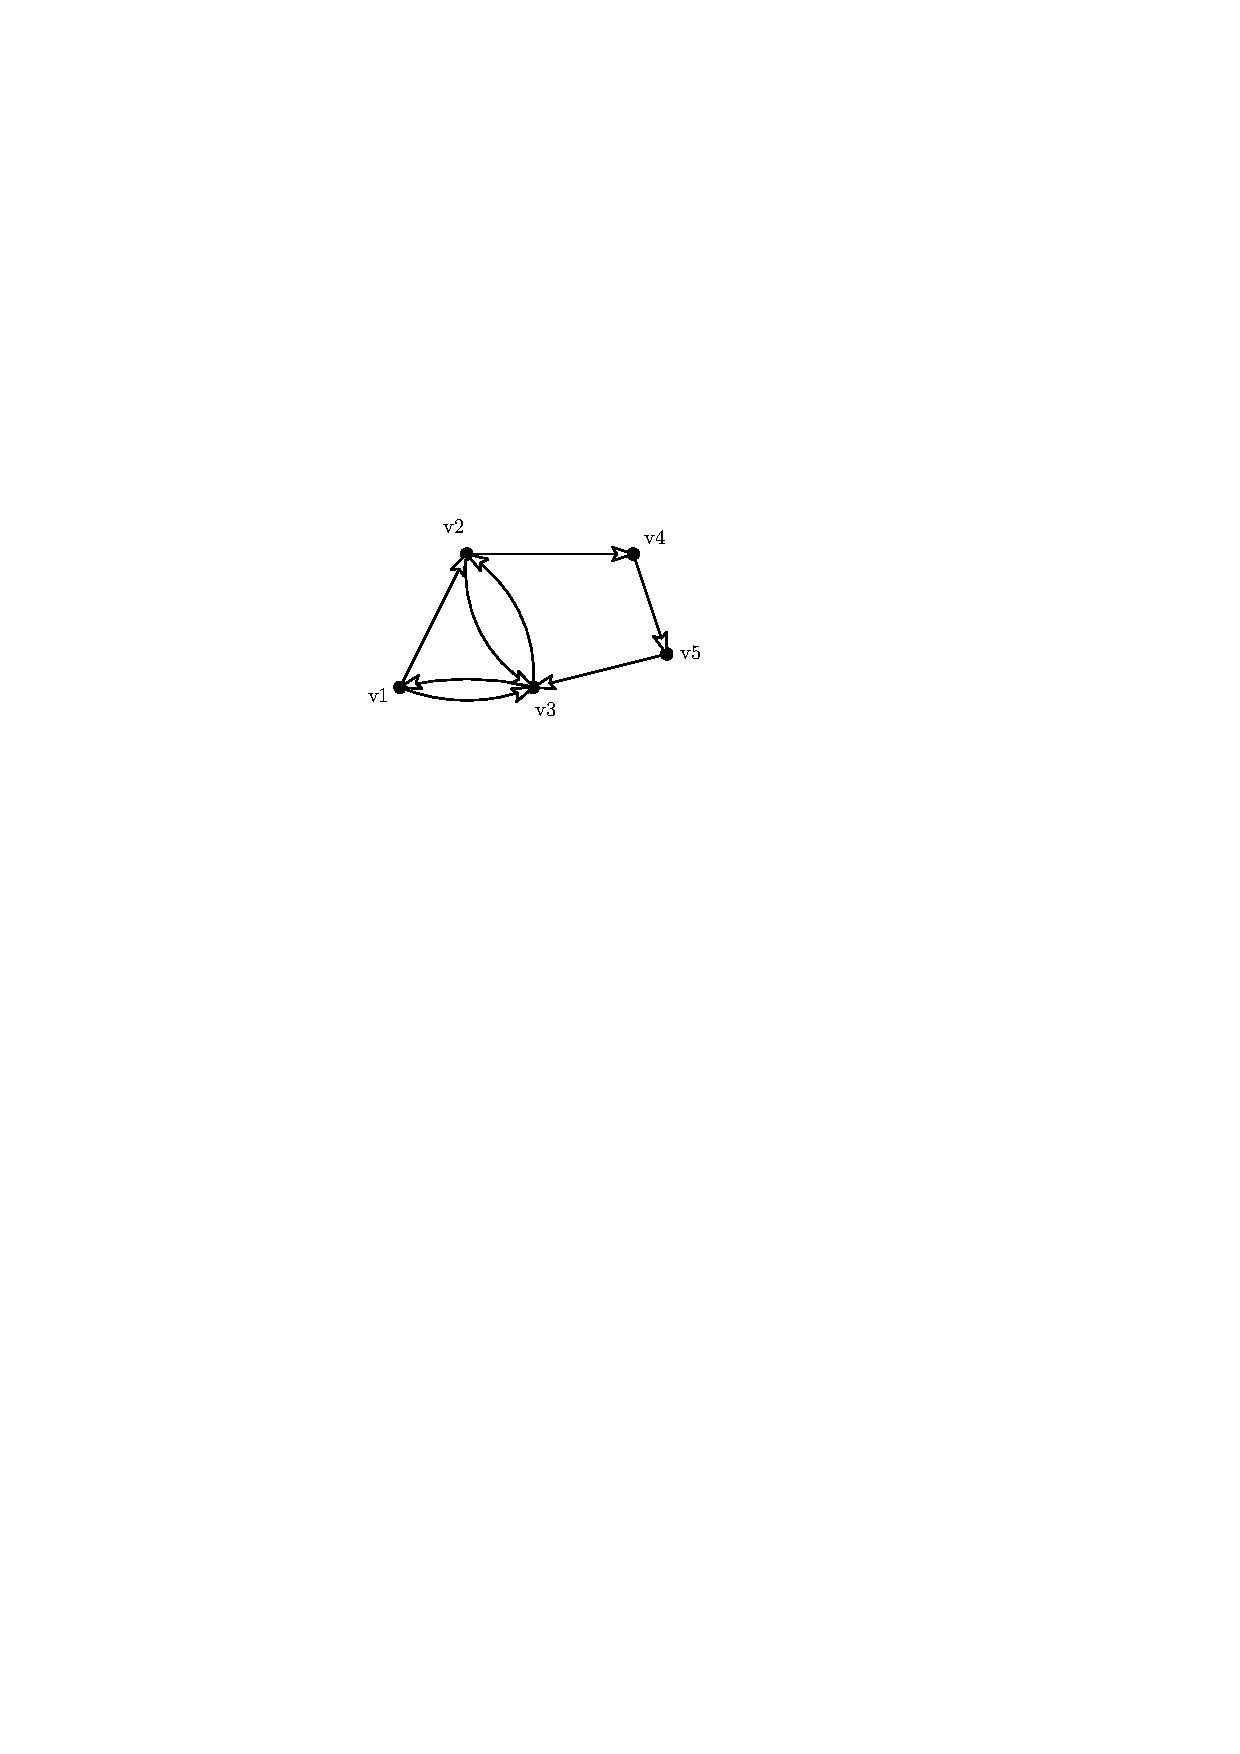
\includegraphics[width = \textwidth]{../media/gerichtet.pdf} \\
\caption{G}
\label{fig:directed}
\end{subfigure}
\begin{subfigure}{0.49\textwidth}
\centering
{
\begin{blockarray}{cccccc}
  & $v_{1}$ & $v_{2}$ & $v_{3}$ & $v_{4}$ & $v_{5}$ \\
\begin{block}{c(ccccc)}
  $v_{1}$ & 0 & 1 & 1 & 0 & 0 \\
  $v_{2}$ & 0 & 0 & 1 & 1 & 0 \\
  $v_{3}$ & 1 & 1 & 0 & 0 & 0 \\
  $v_{4}$ & 0 & 0 & 0 & 0 & 1 \\
  $v_{5}$ & 0 & 0 & 1 & 0 & 0 \\
\end{block}
\end{blockarray}
}
\vspace{0.1cm}
\caption{Adjazenzmatrix von G}
\label{mx:directed}
\end{subfigure}
\caption{Ein gerichteter Graph G und seine Adjazenzmatrix}
\label{directedGraph}
\end{figure}

\subsubsection{Gewichtete Graphen}
In dieser Arbeit bezeichnet der Begriff \textit{gewichteter Graph} einen \textit{Kanten}gewichteten Graphen, bei dem jeder Kante ein Wert ~$c$ zugewiesen wird.

$$G = (V,E)$$ 
\begin{center}
mit
\end{center}
$$c: E \rightarrow \mathbb{R}$$

Neben dem Kantengewichteten gibt es auch \textit{Ecken}gewichtete Graphen, bei welchen entsprechend die Ecken gewichtet werden.
Gewichtete Graphen können gerichtet und ungerichtet sein.
Ein klassisches Beispiel hierfür ist der Linien-Netzplan einer Straßenbahn, bei dem die Ecken einzelne Haltestellen darstellen und die Kantengewichte die benötigten Minuten beinhalten.

\begin{figure}[htb]
\centering
\begin{subfigure}{0.49\textwidth}
\centering
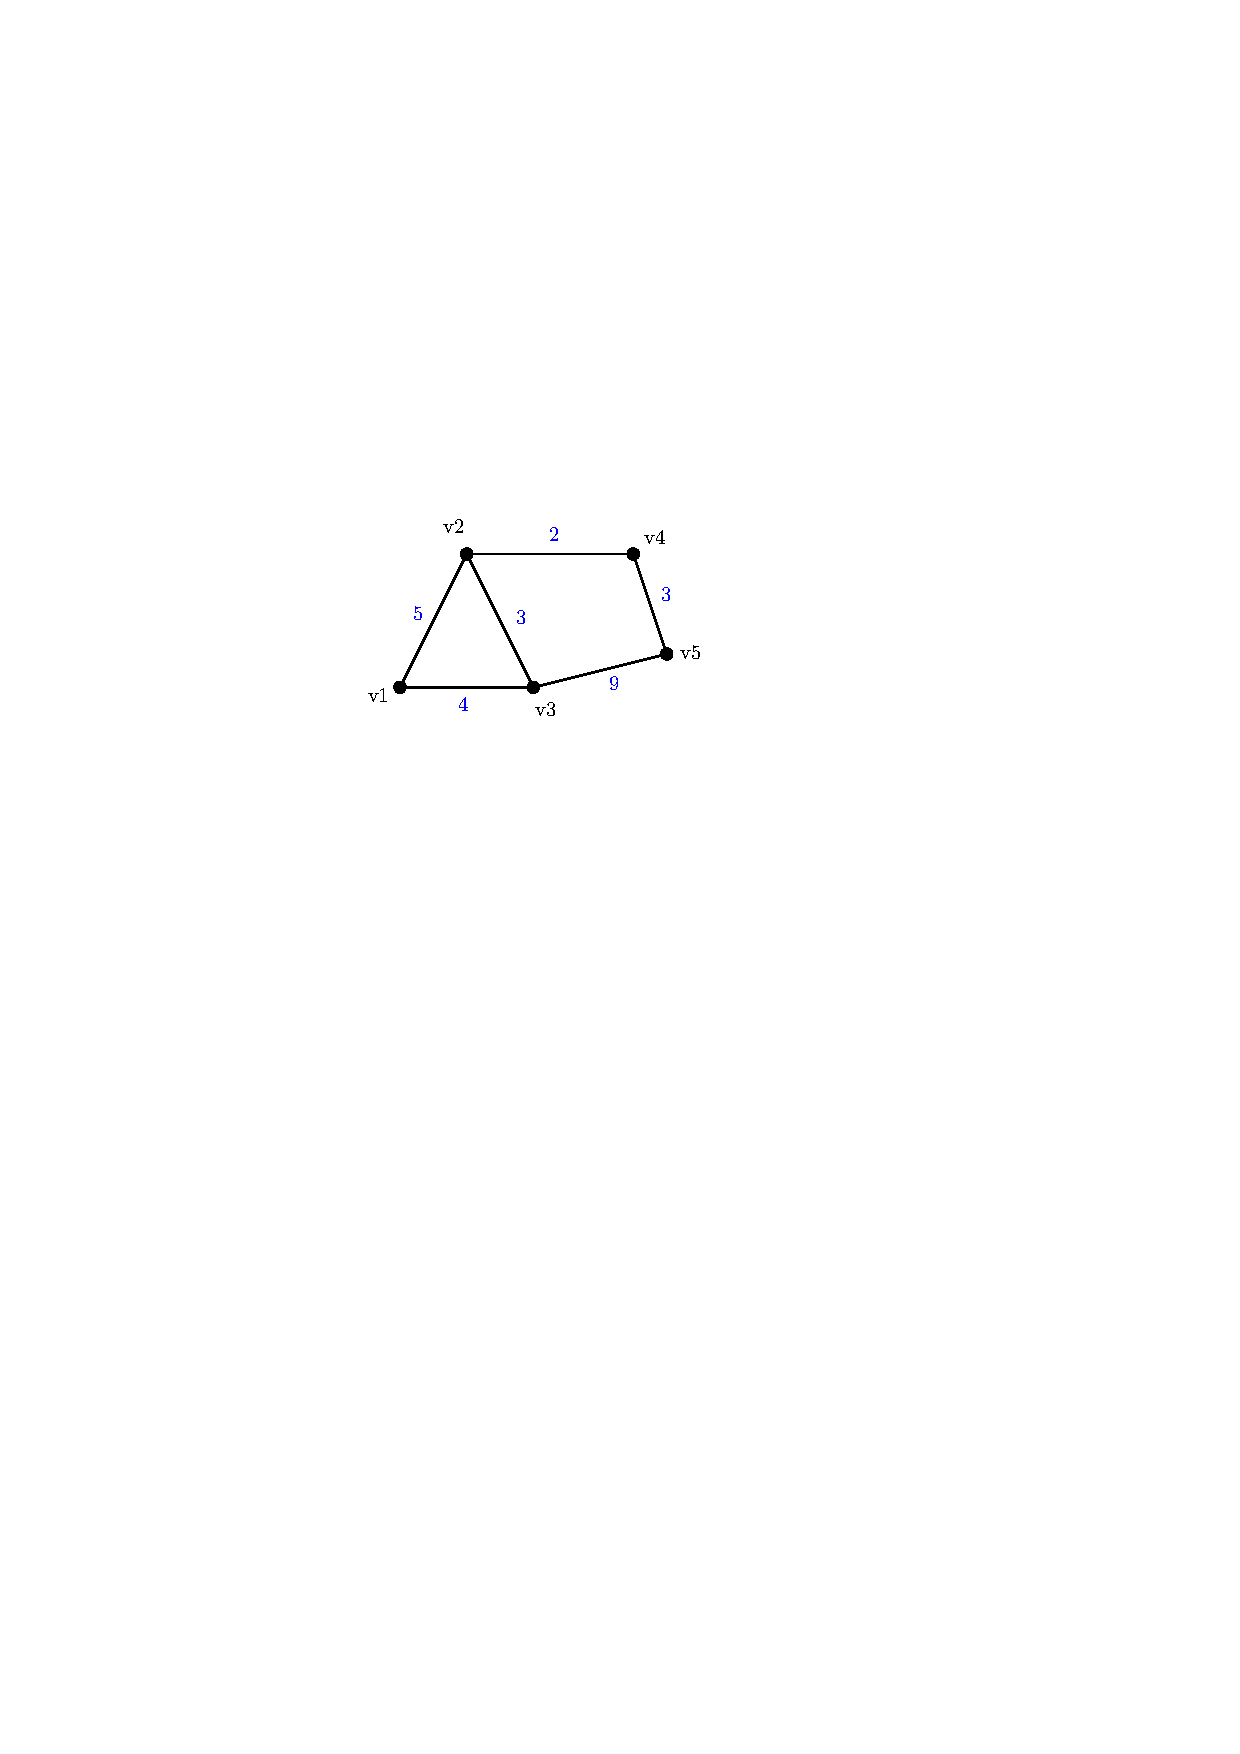
\includegraphics[width = \textwidth]{../media/gewichtet.pdf} \\
\caption{G}
\label{fig:weighted}
\end{subfigure}
\begin{subfigure}{0.49\textwidth}
\centering
{
\begin{blockarray}{cccccc}
  & $v_{1}$ & $v_{2}$ & $v_{3}$ & $v_{4}$ & $v_{5}$ \\
\begin{block}{c(ccccc)}
  $v_{1}$ & 0 & 5 & 4 & 0 & 0 \\
  $v_{2}$ & 5 & 0 & 3 & 2 & 0 \\
  $v_{3}$ & 4 & 3 & 0 & 0 & 9 \\
  $v_{4}$ & 0 & 2 & 0 & 0 & 3 \\
  $v_{5}$ & 0 & 0 & 9 & 3 & 0 \\
\end{block}
\end{blockarray}
}
\vspace{0.1cm}
\caption{Adjazenzmatrix von G}
\label{mx:weighted}
\end{subfigure}
\caption{Ein gewichteter Graph G und seine Adjazenzmatrix}
\label{weightedGraph}
\end{figure}

Mit gewichteten Graphen können diverse Problemstellungen gelöst werden, zum Beispiel die Bestimmung maximaler (Durch-)Flüsse in Rohrsystemen oder das Berechnen kürzester Wege.
Andererseits kann ein gewichteter Graph auch für Routing-Zwecke eingesetzt werden, indem räumliche Positionen sowie Eigenschaften von Straßen in der Datenstruktur eines Graphen gespeichert werden.

\subsubsection{Erstellung eines Graphen aus OpenStreetMap-Daten}
\label{sec:osmgraph}

Die \gls{osm}\footnote{OpenStreetMap ist ein 2004 gegründetes internationales Projekt mit dem Ziel, eine freie Weltkarte zu erschaffen (\href{www.openstreetmap.de}{www.openstreetmap.de}). Die Daten werden von vielen Freiwilligen auf der ganzen Welt generiert und in einer Datenbank unter der Open Database Lizenz zur verfügung gestellt.} Datenstruktur kann als Graph abgebildet werden.
Hier werden Punktobjekte als \textit{Nodes} (Ecken) und Linienobjekte als \textit{Ways} (Kanten) bezeichnet.
Ein Way ist dabei die Verbindung zwischen zwei oder mehreren Nodes.
Zusätzlich gibt es \textit{Relations} (Relationen) die einer Menge aus Nodes und Ways einen funktionalen Zusammenhang zuschreiben.
Für Straßennetze kann dies durchaus hilfreich sein, um beispielsweise unterschiedliche Segmente eines Autobahnabschnittes zusammenzufassen oder um Abbiegevorschriften an Kreuzungen zu beschreiben (\cite{osmrelation}).

Um aus den \gls{osm} Daten einen routingfähigen Graphen zu erhalten, müssen zuerst alle benutzbaren Nodes und Ways extrahiert werden.
Diese werden anhand ihrer \gls{osm}-Tags identifiziert.
Dazu gehören alle Arten von Straßen und Wegen, sowie als befahrbar gekennzeichnete Ways (beispielsweise asphaltiert, aber ohne angegebenen Straßentyp).
Für das Routing sind vor allem Verbindungspunkte wie Kreuzungen, Ab- und Auffahrten sowie Sackgassen, wichtig.
Diese sogenannten \textit{Tower Nodes} werden daher aus den importierten Daten ermittelt.
Anschließend werden die Straßen anhand der Verbindungspunkte segmentiert.
Danach werden die Verbindungen zwischen den Tower Nodes berechnet und anhand der Distanz gewichtet.
Das Grundgerüst des eigentlichen Routing-Graphen ist damit erstellt.
Einbahnstraßen und Abbiegevorschriften werden berücksichtigt und geben die Richtung der Kanten an (\cite{osmgraph}).
Die Punkte zwischen zwei Tower Nodes werden \textit{Pillar Nodes} genannt.
Sie werden als \textit{WayGeometry} auf der jeweiligen Kante gespeichert, da sie nicht für das berechnen der Route benötigt werden (Abb.~\ref{fig:tower}).
Das Routing ist dadurch um ungefähr das 8-fache schneller (\cite{graphhopper}).
Relevante Attribute wie Geschwindigkeit oder Straßentyp werden vereinheitlicht und als \textit{Flags} (Markierungen) auf der Kante gespeichert.
Diese sind für die individuelle Gewichtung bei der Routenfindung interessant.
(Mehr zu Gewichtung später in Kapitel ~\ref{backendGraphBuild}).
Zuletzt wird der Graph abgespeichert und ist für Routing Abfragen bereit (\cite{osmgraph}).

\begin{figure}[htb]
\centering
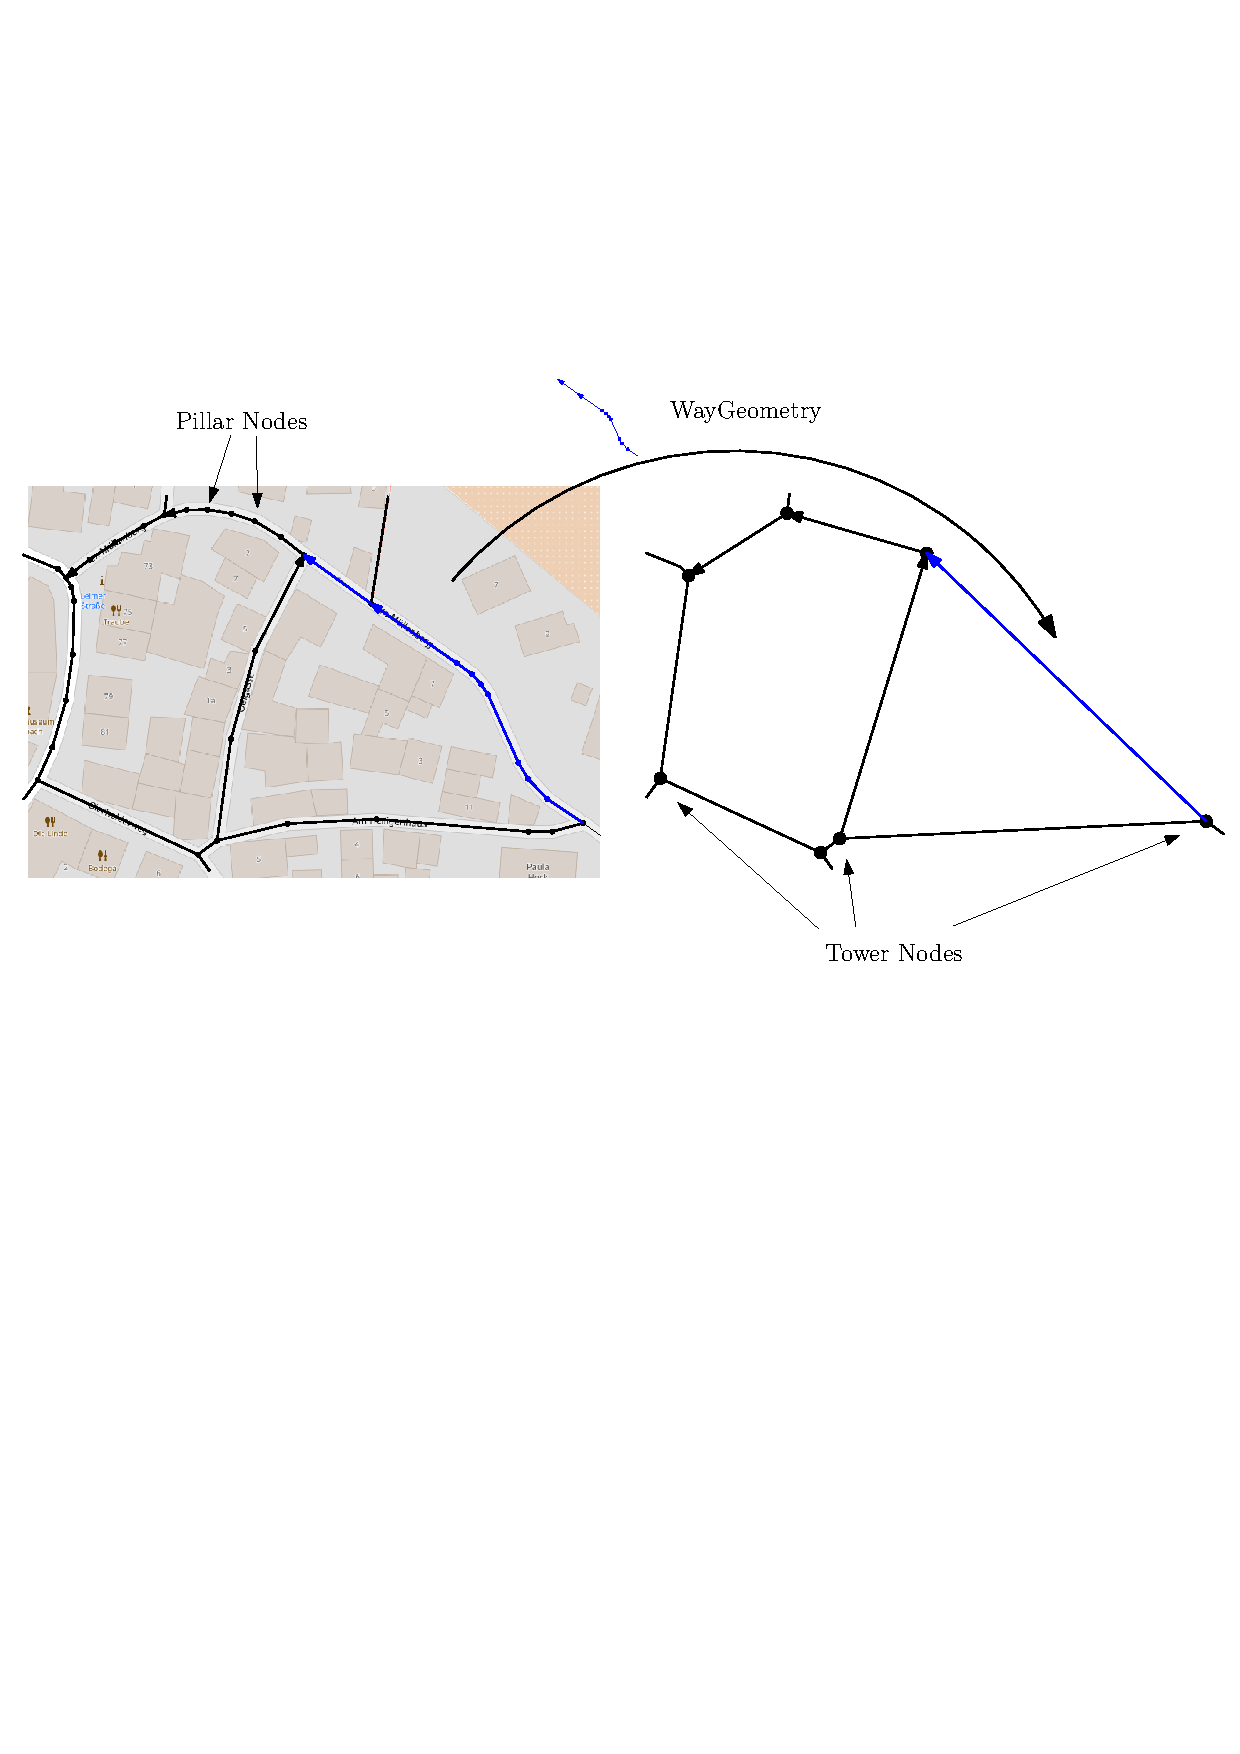
\includegraphics[width = \textwidth]{../media/towers.pdf} \\
\caption[Simplifizierung eines \gls{osm} Datensatzes]
{\centering Simplifizierung eines \gls{osm} Datensatzes
\par\justifying\scriptsize
Bei der Erstellung des routingfähigen Graphen wird der Verlauf eines Wegsegmentes(\textit{Pillar Nodes}) aus den OSM-Daten als \textit{WayGeometry} auf der Kante des Graphen für spätere Abfragen gespeichert. Übrig bleibt der aus \textit{Tower Nodes}(Kreuzungen, Abbiegungen und Sackgassen bestehende) bestehende Graph.
}
\label{fig:tower}
\end{figure}

\subsection{Routing}

Routing bezeichnet den Vorgang in einem Netzwerk Wege zu finden, auf denen Daten entlang gesendet werden können.
Diese Definition bezieht sich vor allem auf elektronische Datennetzwerke wie das Telefonnetz oder das Internet.
Im Fachbereich der Geoinformationssysteme werden hauptsächlich Straßennetze für Routing-Analysen verwendet (\cite[165]{handbook}).
Ein Weg \textit{P} (\textit{engl: path}) von einer Startecke ~$s$ zu einer Zielecke ~$z$ ist eine Folge von benachbarten Ecken, mit $s~$ als erste Ecke und $z~$ als letzte Ecke der Folge.
Die Weglänge entspricht in einem gewichteten Graphen der Summe aller Kantengewichte.

Eine der wichtigsten Netzwerk-Analyse-Operationen ist die Berechnung des kürzesten Weges zwischen zwei Ecken.
Jedes Navigationssystem muss diese Aufgabe erfüllen können.
Der kürzeste Weg hat demnach die Eigenschaft, dass die Summe aller Kantengewichte, in anderen Worten die Kosten des Weges, minimal gegenüber allen anderen Wegen im Graphen ist.

\subsubsection{Shortest Path Problem}
Die nächstliegendste zu beleuchtende Problemstellung ist das \textit{Shortest Path Problem} welches aber nicht mit dem \textit{\gls{tsp}} verwechselt werden sollte.
Beim \gls{tsp} ist die kürzeste Tour auf einem Graphen gesucht, die jede Ecke des Graphen besucht (\cite[135]{algorithms}).
Das Shortest Path Problem lässt sich in drei Typen untergliedern denen jeweils ein gerichteter Graph $G = (V,E)$ mit der Gewichtsfunktion $c: E \rightarrow \mathbb{R}$ zugrunde liegt.
Beim \textit{\gls{spp}} wird der kürzeste Weg von einer Ecke $a~$ zu einer anderen Ecke $b~$ mit $a,b\in V$ gesucht.
Beim \textit{\gls{ssp}} wird der kürzeste Weg einer Ecke $a~$ zu jeder anderen Ecke ermittelt.
Das \textit{\gls{apsp}} sucht den kürzesten Weg von jeder Ecke zu jeder anderen Ecke in $V~$ (\cite[169\psq]{algorithms}).

Für eine Route von Startecke $s~$ zur Zielecke $z~$ ist das \gls{spp} demnach die richtige Wahl.
Allerdings wird dazu das \gls{ssp} herangezogen, welches mit dem Algorithmus von Dijkstra gelöst werden kann.


\subsubsection{Dijkstra-Algorithmus}
\label{sec:dijkstra}
Der von Dijkstra entwickelte Algorithmus (\cite{dijkstra}) benötigt einen gewichteten Graphen ohne negative Kantengewichte\footnote{Das Problem bei Graphen mit negativer Gewichtung entsteht, wenn diese auf einer Schlinge oder der Kante eines Rings liegen.
Sobald der Algorithmus den Zyklus erreicht, werden die Kosten für die Ecken des Zyklus immer geringer.
Die Kosten für den kürzesten Weg nähern sich $-\infty $ während der Algorithmus in einer Endlosschleife läuft.
Deswegen ist der Dijkstra nur für positive Kantengewichte anwendbar (\cite[194\psq]{kurt})}, sowie eine Startecke $s \in V$.
Es gibt eine Warteliste $W_{s}$ mit unmarkierten \textit{gesichteten} Ecken.
Dort sind für alle $v~$ die Kosten für den bisher kürzesten Weg von $s~$ und die jeweilige vorangehende Ecke auf diesem Weg gespeichert.
Die Kosten können sich ändern, wenn ein noch kürzerer Weg gefunden wird.
Diese Liste enthält zu Beginn nur den Startpunkt $s~$ mit den trivialen Kosten $0~$.
In einer weitere Liste werden die endgültig kürzesten Wege $K_{s}$ aller markierten Ecken gespeichert.

Dijkstra's Algorithmus markiert die Ecke mit den geringsten Kosten aus $W_{s}$ und verschiebt diese nach $K_{s}$.
Nun werden alle benachbarten Ecken gesichtet und die Kosten berechnet.
Die Kosten und der Vorgänger (die zuletzt markierte Ecke) werden in $W_{s}$ gespeichert.
Die Ecke mit den geringsten Kosten wird als nächstes markiert, da der Weg dorthin auf jeden Fall ein kürzester ist.
Dieser Vorgang wird wiederholt bis alle Ecken aus $W_{s}$ markiert wurden und $W_{s}$ somit leer ist.

% Init Dijkstra
\begin{figure}[htb]
\centering
\begin{subfigure}{0.49\textwidth}
\centering
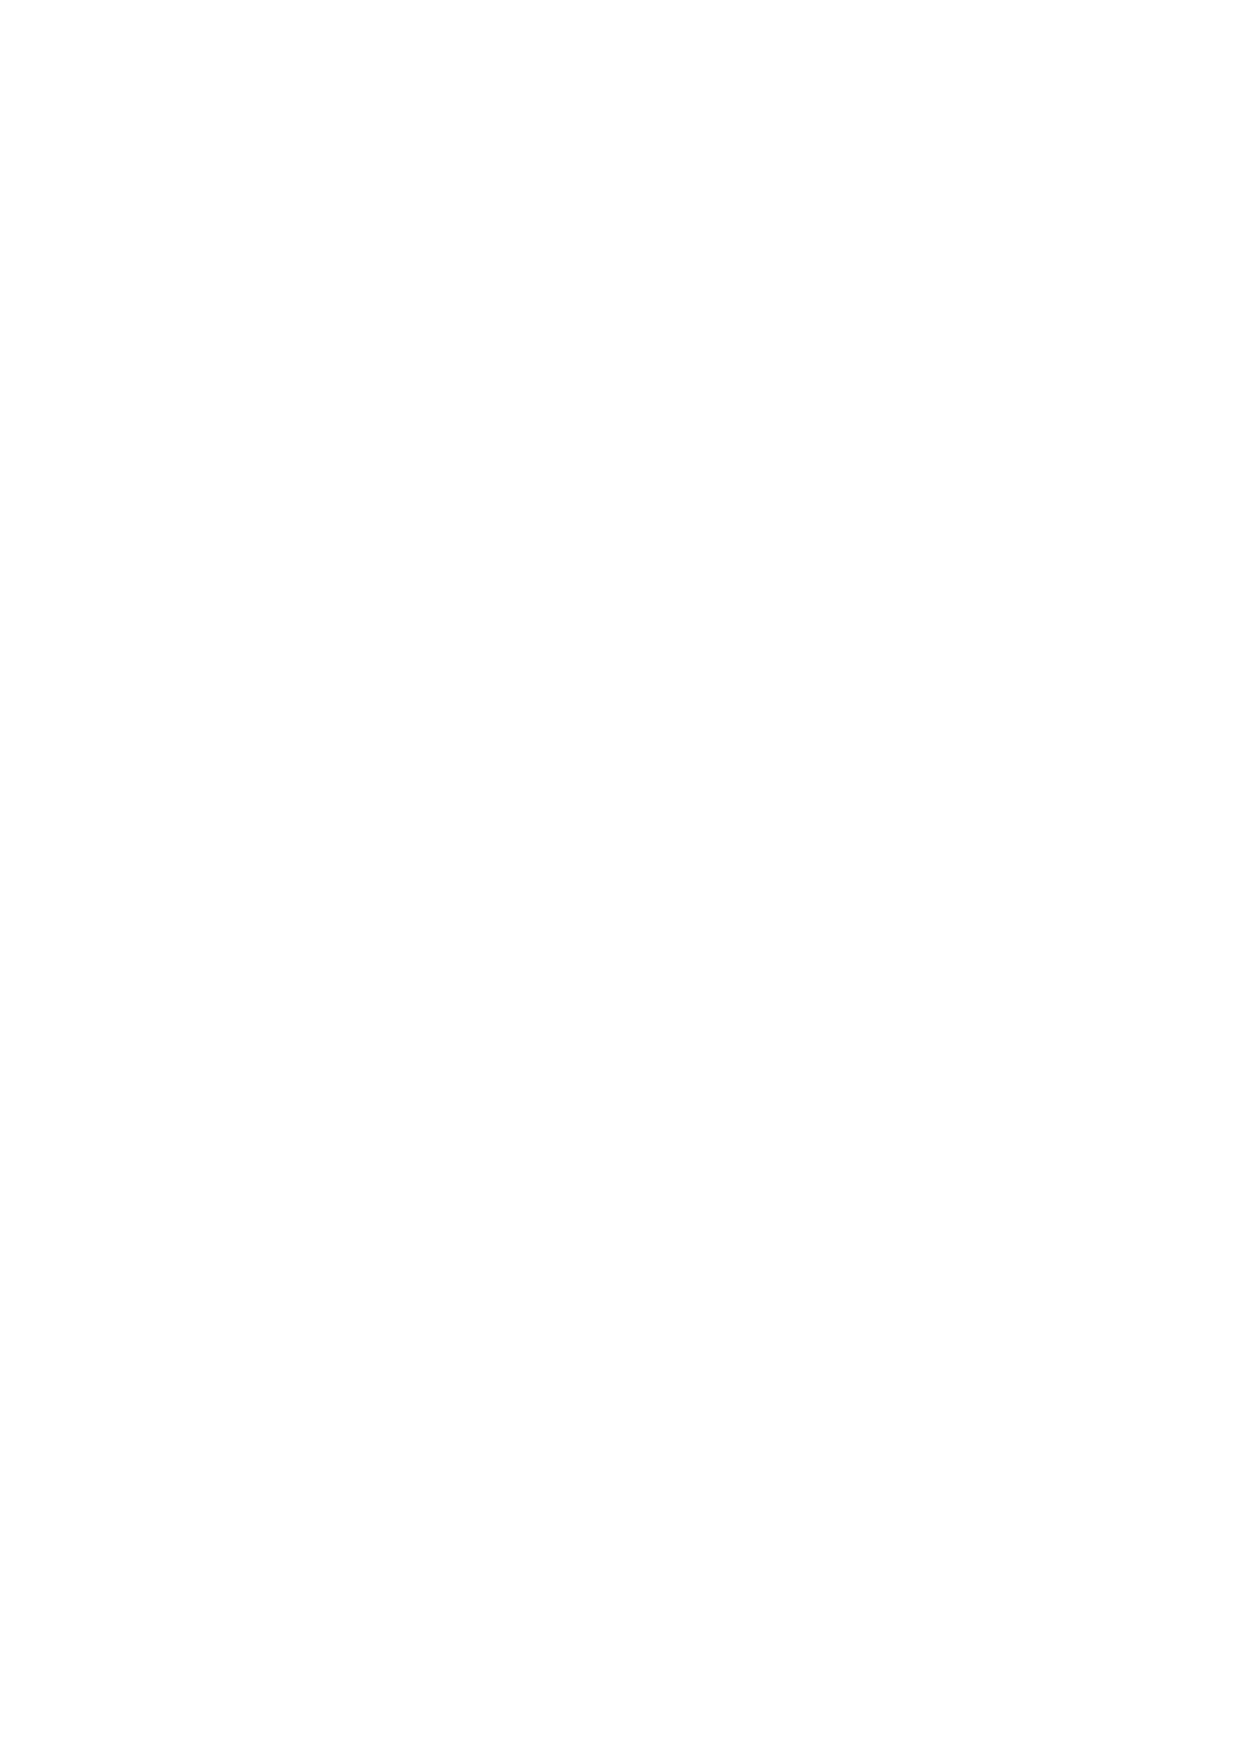
\includegraphics[width = \textwidth]{../media/dijkstra.pdf} \\
\caption{G}
\label{fig:dijkstra}
\end{subfigure}
\begin{subfigure}{0.49\textwidth}
\centering
{
\begin{blockarray}{cccccc}
  & $v_{1}$ & $v_{2}$ & $v_{3}$ & $v_{4}$ & $v_{5}$ \\
\begin{block}{c(ccccc)}
  $v_{1}$ & 0 & 5 & 4 & 0 & 0 \\
  $v_{2}$ & 7 & 0 & 0 & 3 & 0 \\
  $v_{3}$ & 4 & 2 & 0 & 0 & 8 \\
  $v_{4}$ & 0 & 3 & 6 & 0 & 1 \\
  $v_{5}$ & 0 & 0 & 8 & 1 & 0 \\
\end{block}
\end{blockarray}
}
\vspace{0.1cm}
\caption{Adjazenzmatrix von G}
\label{mx:dijkstra}
\end{subfigure}
\caption{Ein gewichteter und gerichteter Graph G}
\label{dijkstraGraph}
\end{figure}

Die Funktionsweise des Dijkstra Algorithmus wird am Graphen~$G$ in Abbildung~\ref{dijkstraGraph} mit der Startecke $s=v_{1}$ veranschaulicht.

Die erste Ecke der Warteschlange ist $s=v_{1}$.
Da $s~$ der einzige Eintrag ist, sind die Kosten automatisch am geringsten.
$s~$ wird von $W_{s}$ nach $K_{s}$ verschoben, markiert und die erreichbaren Ecken gesichtet.
Das sind $v_{2}$ mit den Kosten $5~$ und $v_{3}$ mit den Kosten $4~$.
Beide werden mit $v_{1}$ als Vorgänger in $W_{s}$ eingetragen.
Im zweiten Durchgang wird $v_{3}$ (geringste Kosten in $W_{s}$) markiert und nach $K_{s}$ verschoben.
Über $v_{3}$ erreichbare Ecken sind $v_{5}$ mit $4+8=12$ Kosten und $v_{2}$ mit $4+2=6$ Kosten.
Da bereits ein kürzerer Weg nach $v_{2}$ besteht, wird der aktuelle Pfad über $v_{3}$ verworfen.
Als nächstes wird $v_{2}$ nach $K_{s}$ verschoben.
Die einzige neue von dort gesichtete Ecke ist $v_{4}$ mit $8~$ Kosten.
Bei der vierten Wiederholung wird $v_{4}$ ($8<12$) markiert.
Es werden $v_{3}$ und $v_{5}$ gesichtet.
Für $v_{3}$ besteht bereits ein kürzerer Weg.
Für $v_{5}$ ist der neue Weg über $v_{4}$ mit den Kosten von $9~$ allerdings kürzer als der Weg über $v_{3}$.
$v_{5}$ wird aktualisiert und der längere Pfad verworfen.
Im fünften Durchgang wird $v_{5}$ als letzte Ecke in $W_{s}$ nach $K_{s}$ verschoben.
Von dort sind keine neuen Ecken sichtbar.
Die Warteschlange ist leer und der Algorithmus damit beendet.

\begin{figure}[htb]
\centering
\begin{subfigure}{0.32\textwidth}
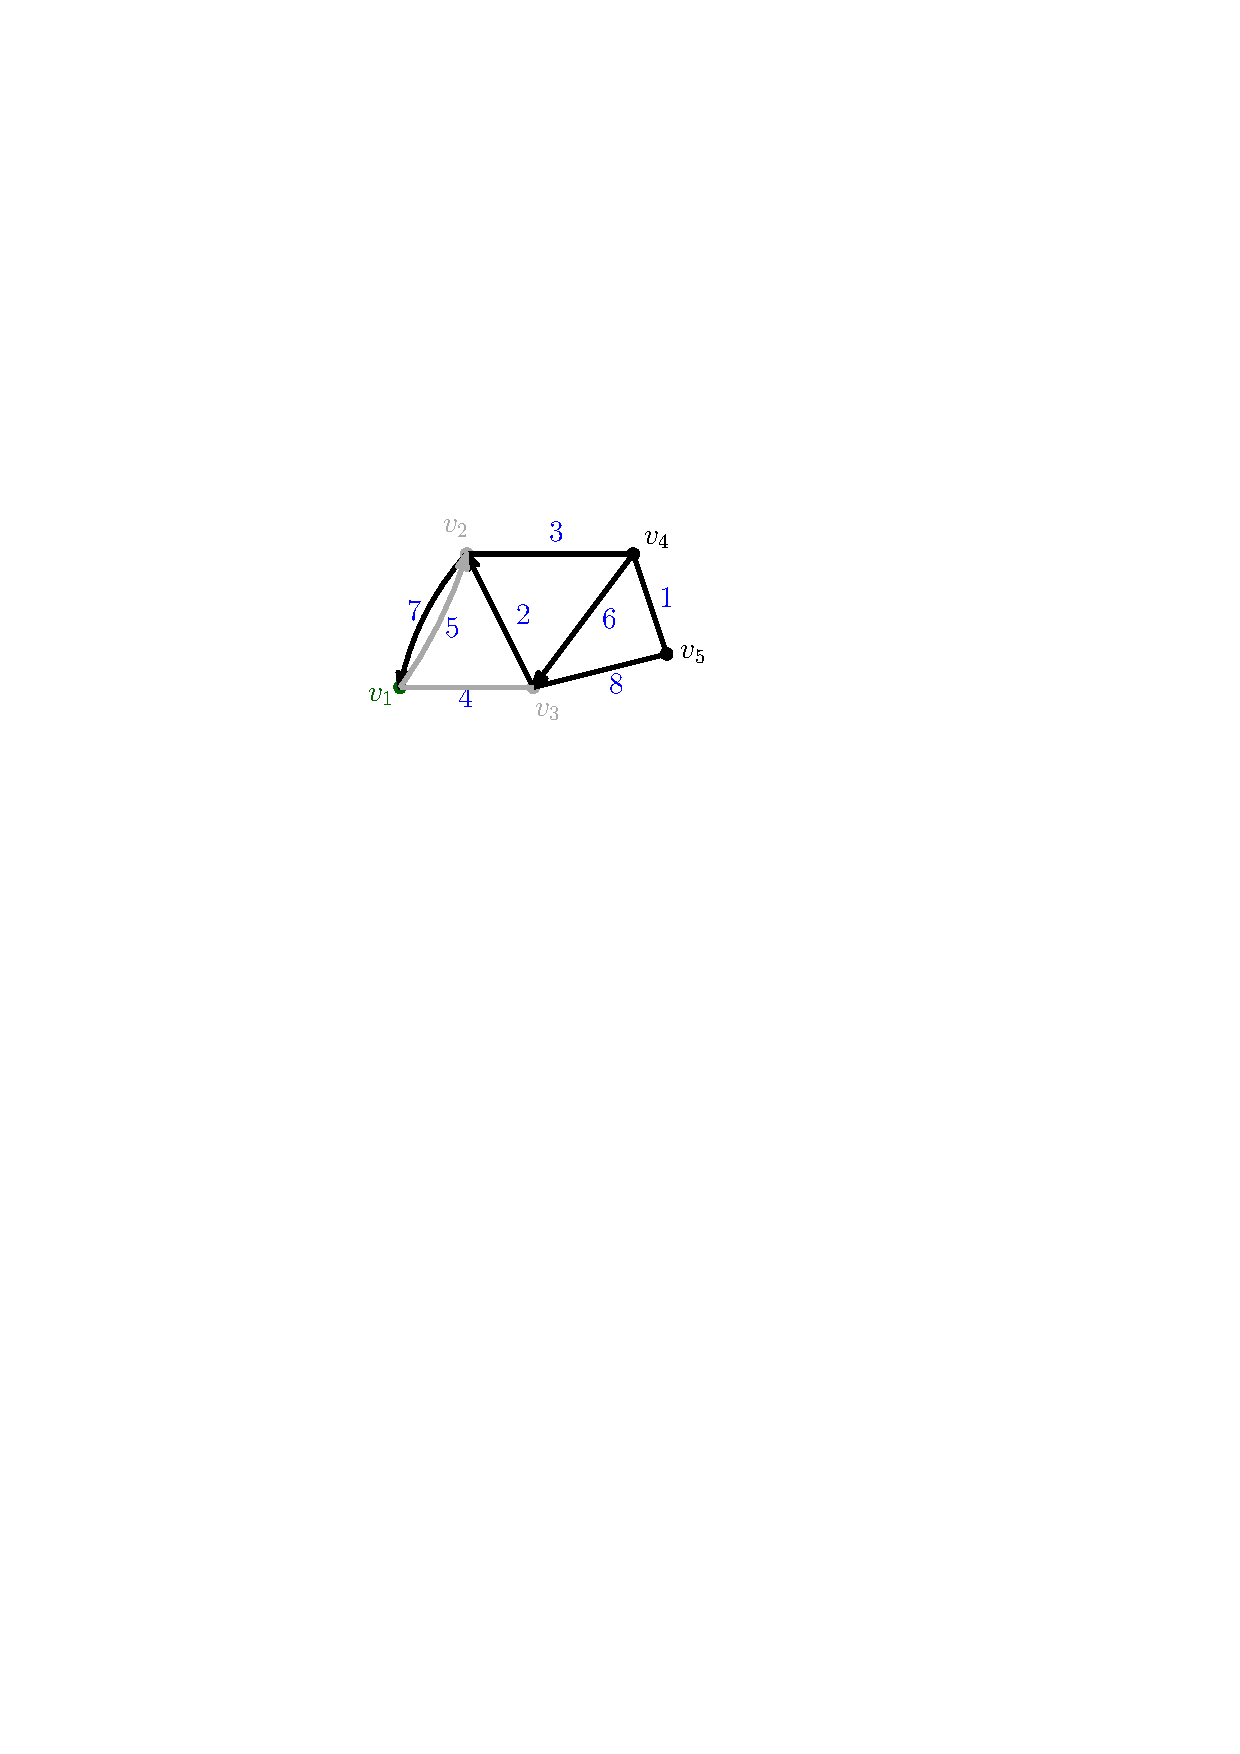
\includegraphics[width = \textwidth]{../media/dijkstra1.pdf} \\
\caption{1. Iteration}
\vspace{0.5cm}
\label{fig:dijkstra1}
\end{subfigure}
\begin{subfigure}{0.32\textwidth}
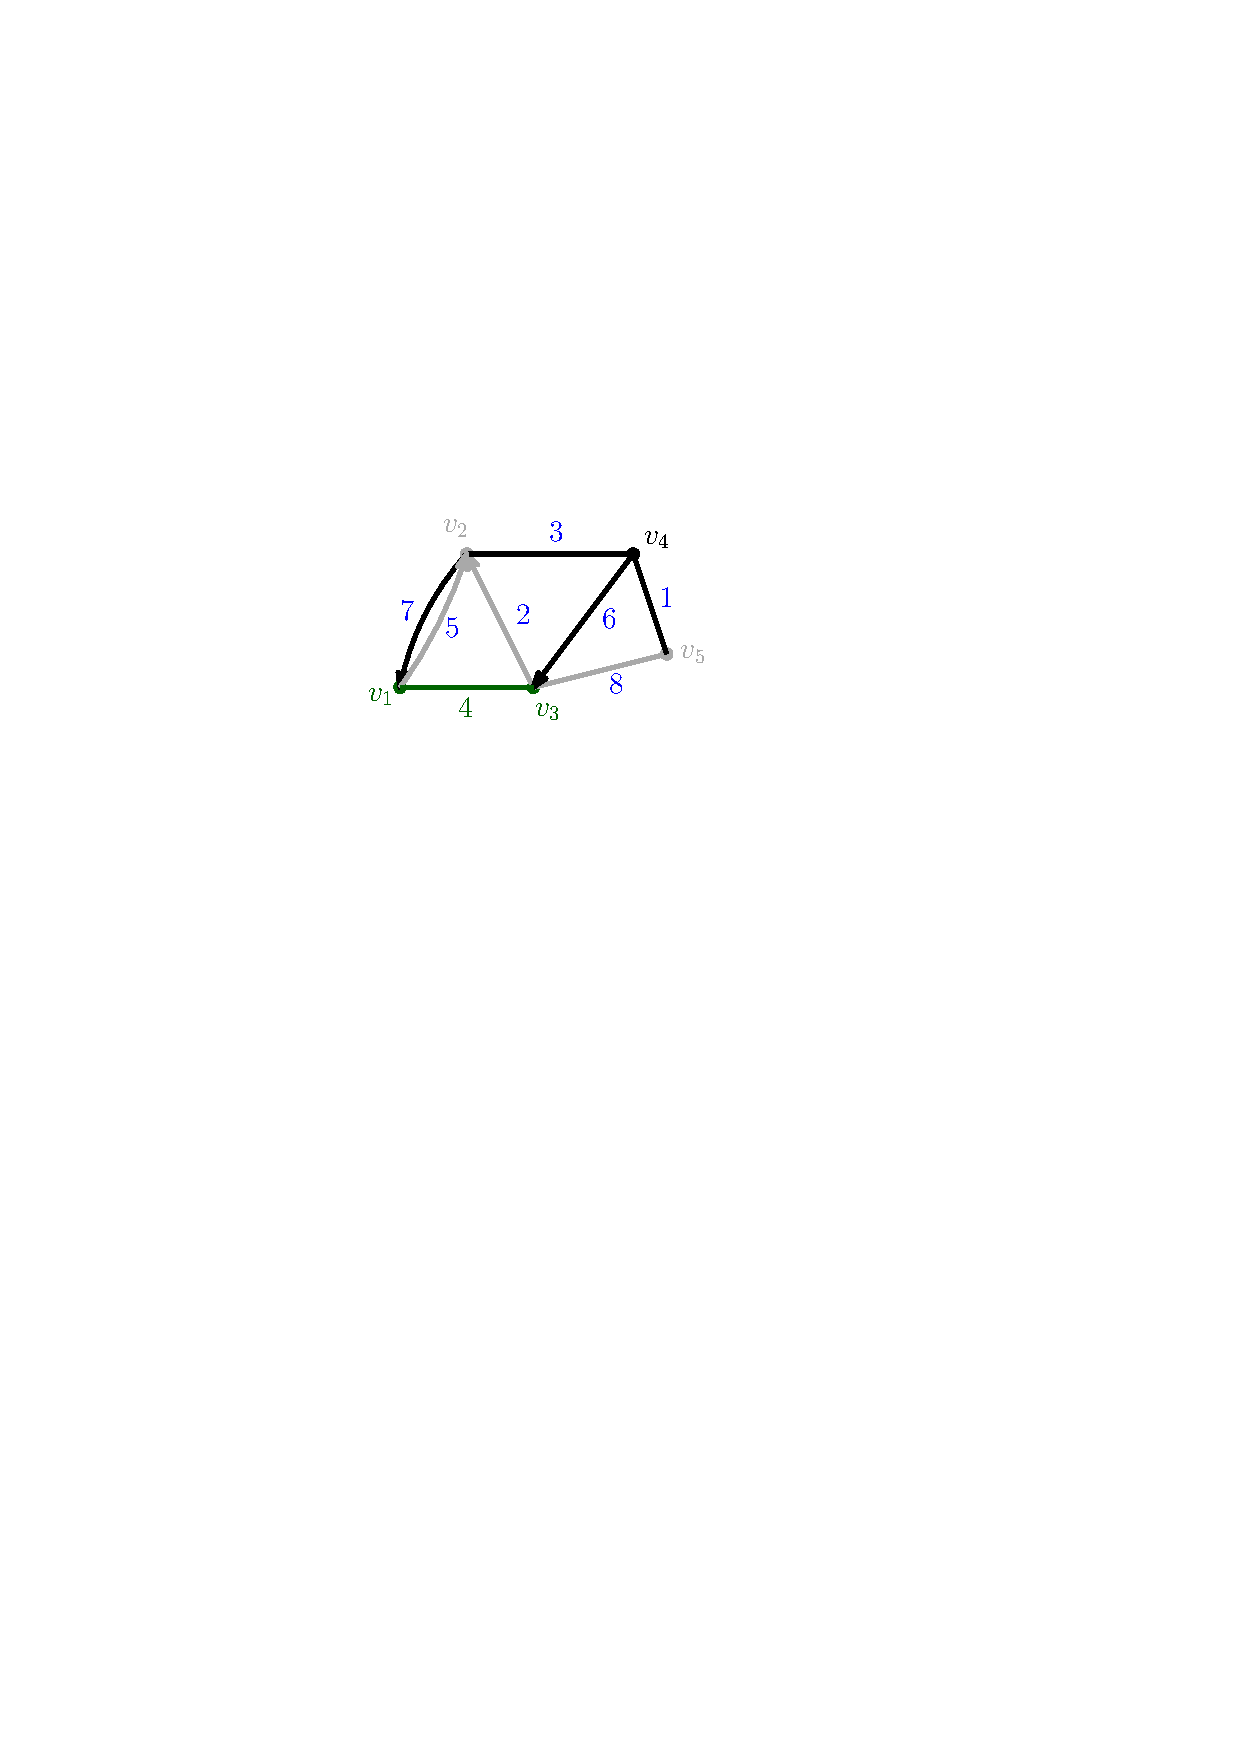
\includegraphics[width = \textwidth]{../media/dijkstra2.pdf} \\
\caption{2. Iteration}
\vspace{0.5cm}
\label{fig:dijkstra2}
\end{subfigure}
\begin{subfigure}{0.32\textwidth}
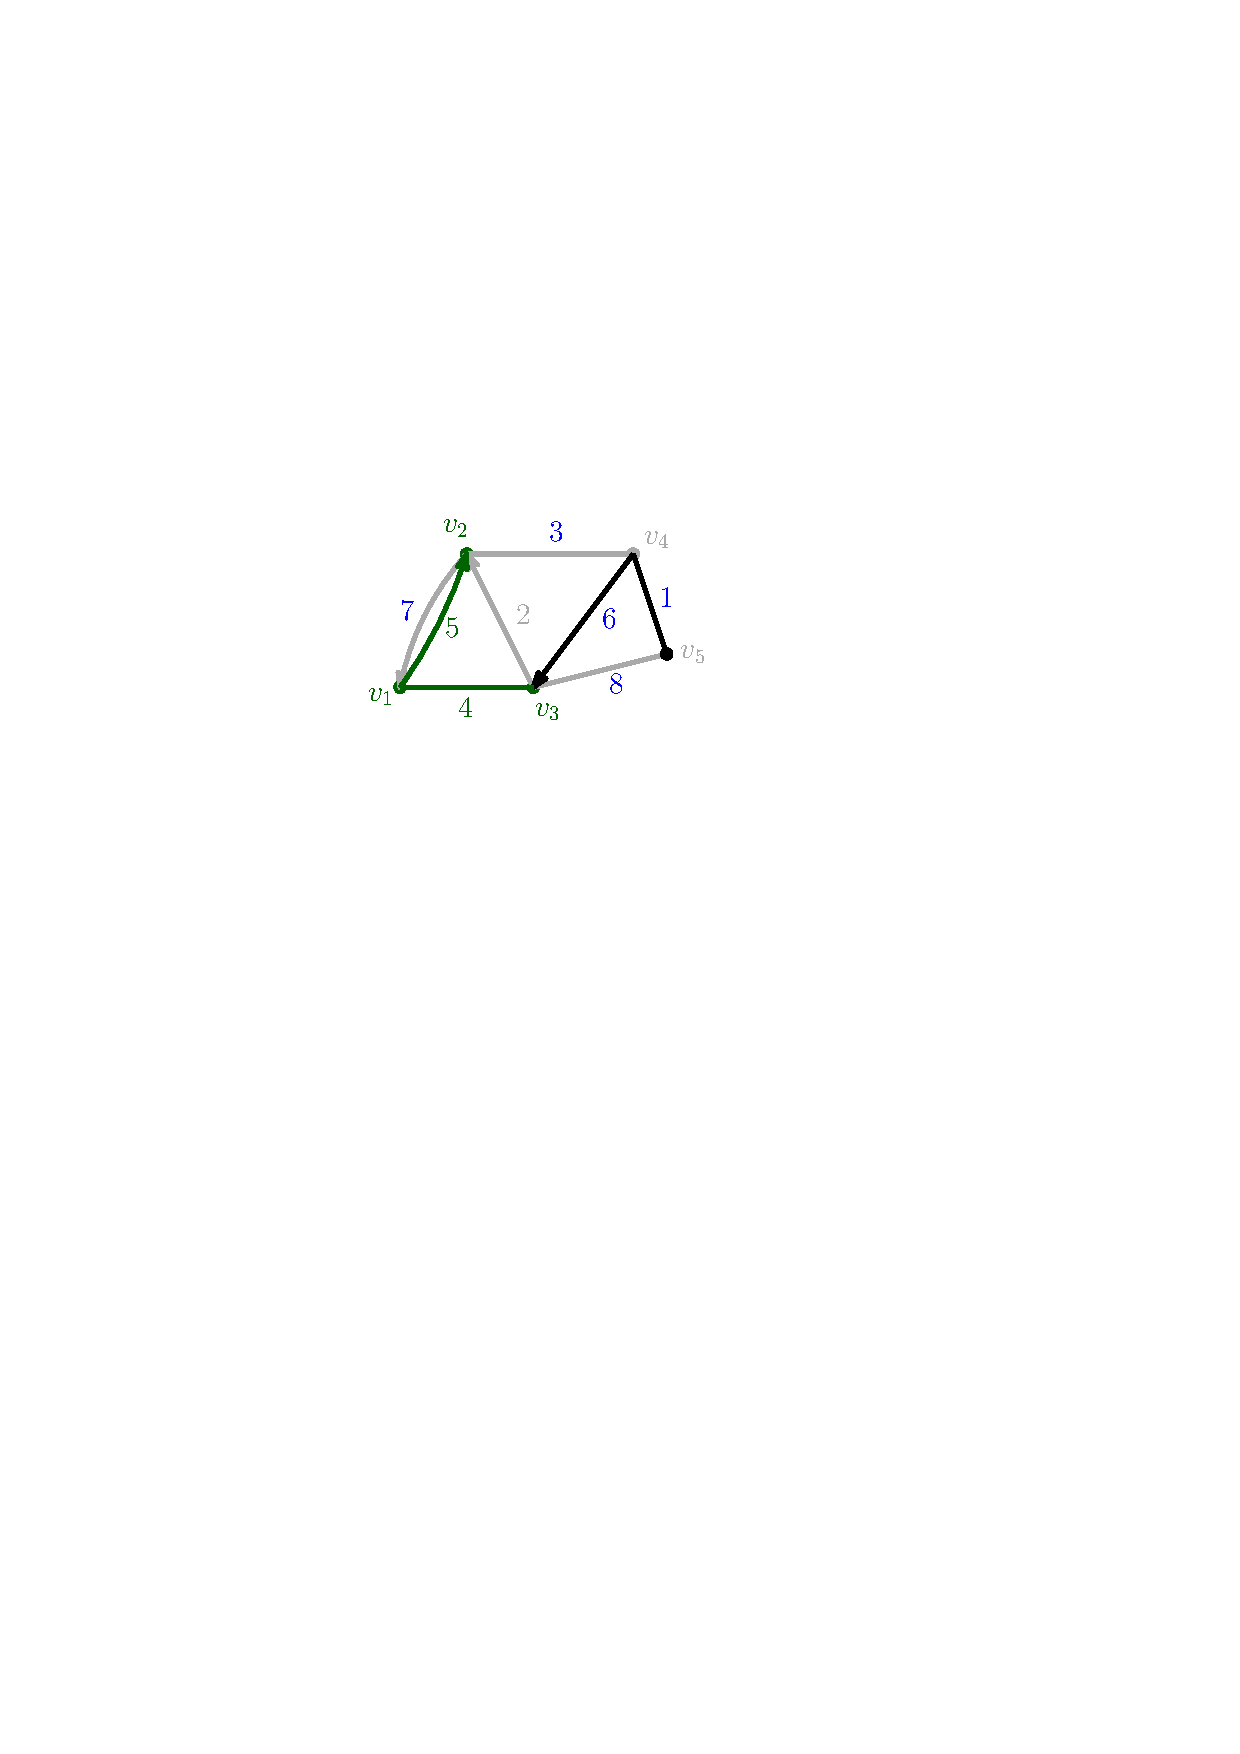
\includegraphics[width = \textwidth]{../media/dijkstra3.pdf} \\
\caption{3. Iteration}
\vspace{0.5cm}
\label{fig:dijkstra3}
\end{subfigure}
\begin{subfigure}{0.32\textwidth}
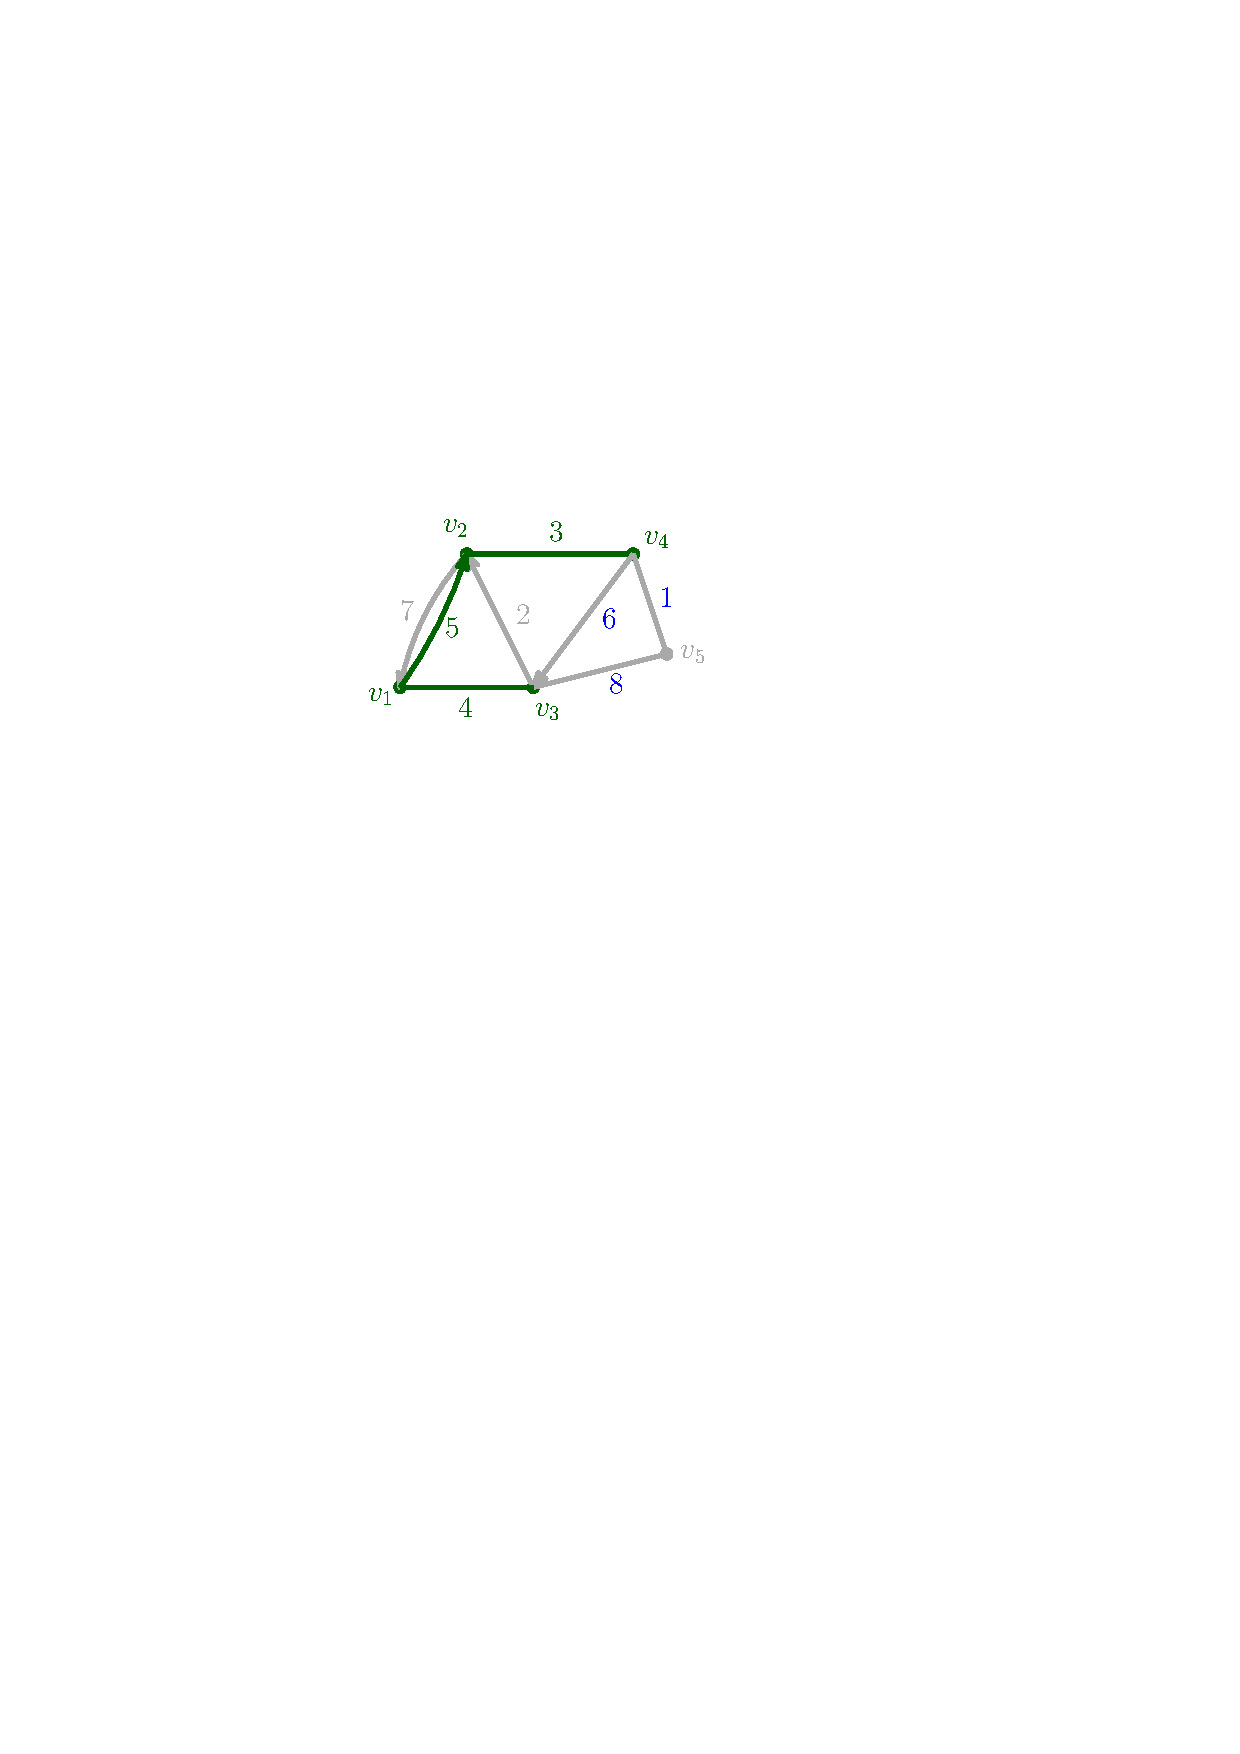
\includegraphics[width = \textwidth]{../media/dijkstra4.pdf} \\
\caption{4. Iteration}
\vspace{0.5cm}
\label{fig:dijkstra4}
\end{subfigure}
\begin{subfigure}{0.32\textwidth}
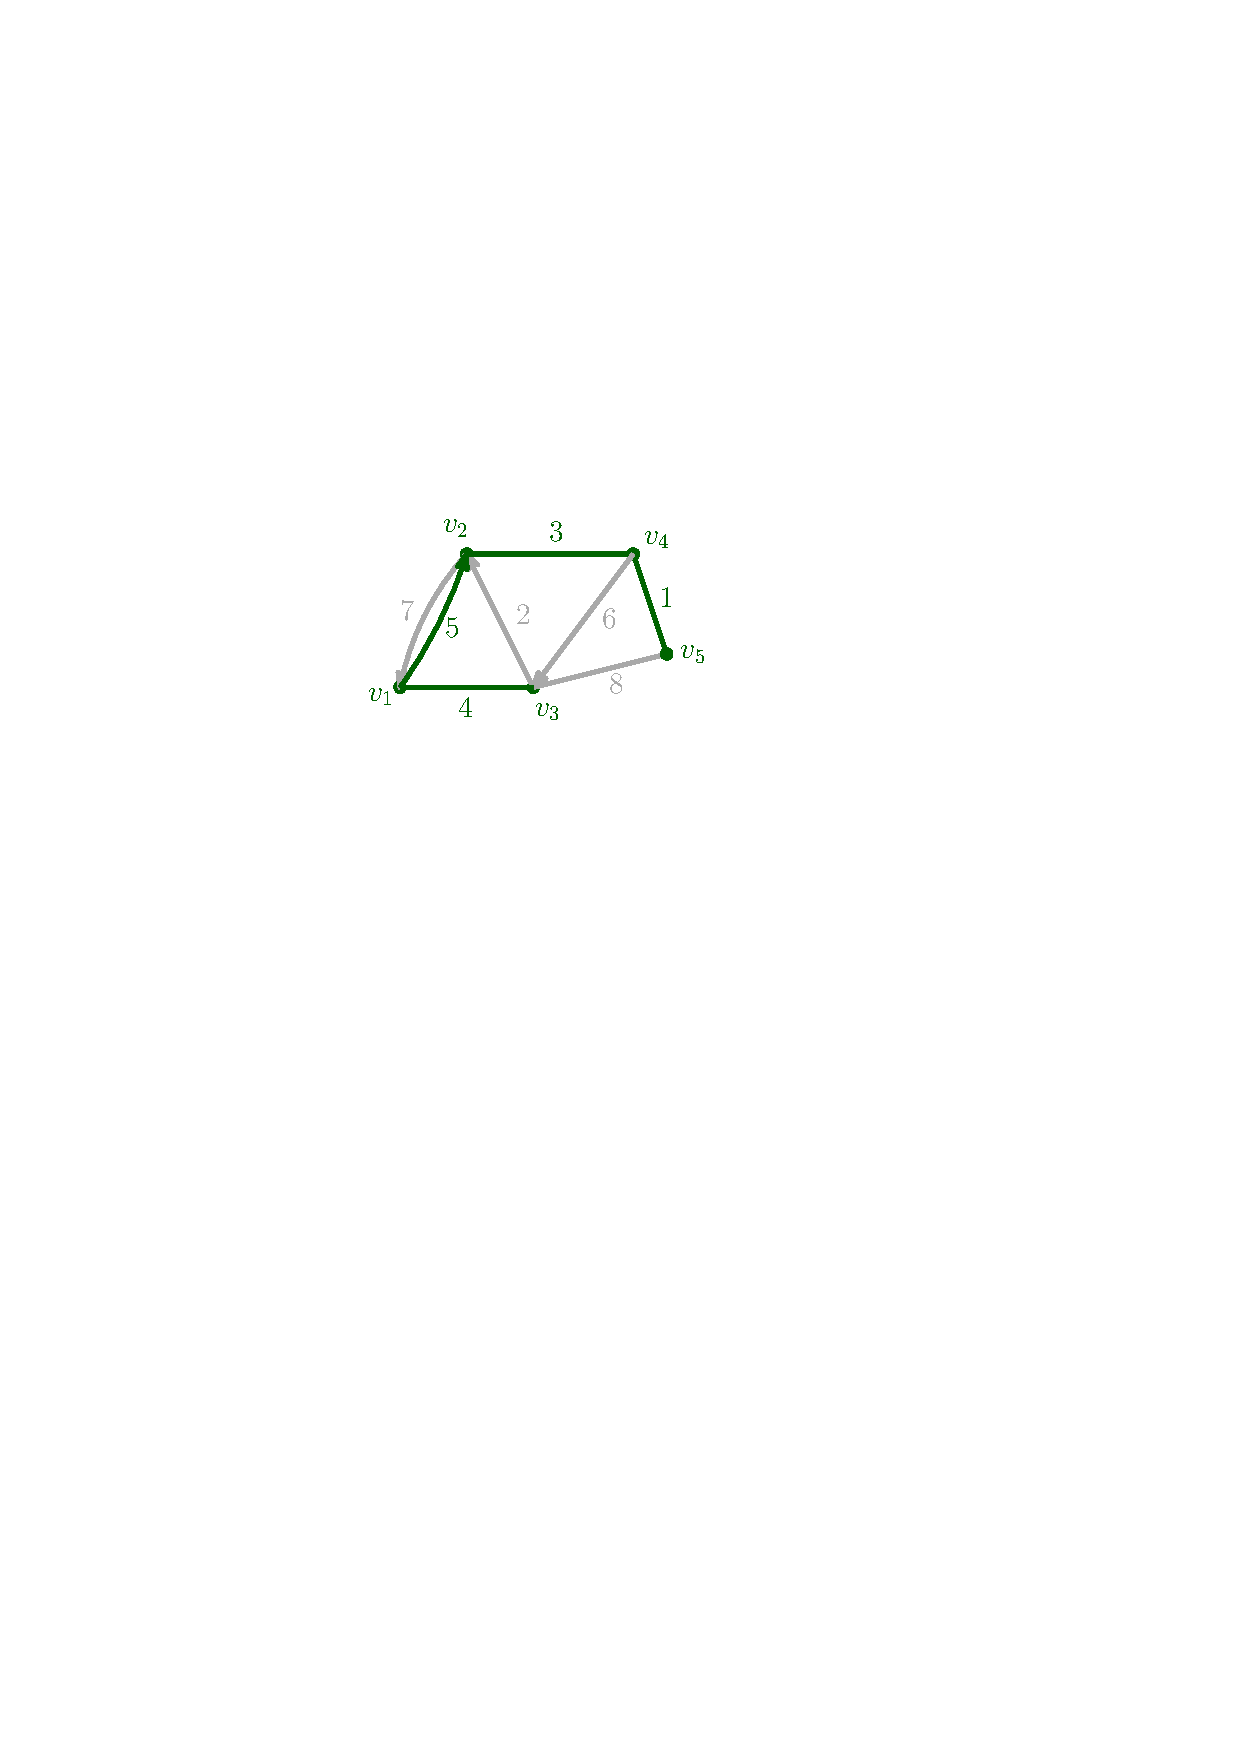
\includegraphics[width = \textwidth]{../media/dijkstra5.pdf} \\
\caption{5. Iteration}
\vspace{0.5cm}
\label{fig:dijkstra5}
\end{subfigure}
\caption[Kompletter Durchlauf eines Dijkstra Algorithmus]
{\centering Kompletter Durchlauf eines Dijkstra Algorithmus
\par\justifying\scriptsize
Der Dijkstra berechnet die kürzesten Wege vom Startpunkt $v_{1}$ zu jeder Ecke des Graphen.
(a) $v_{1}$ wird auf erreichbare Ecken untersucht ($v_{2}$ und $v_{3}$).
(b) Der kürzeste Weg führt zu $v_{3}$. Von $v_{3}$ erreichbare Ecken werden betrachtet.
(c) Aus den möglichen Wegen $v_{1}v_{3}v_{5}$, $v_{1}v_{3}v_{2}$ und $v_{1}v_{2}$ ist der direkte weg nach $v_{2}$ der kürzeste.
$v_{3}v_{2}$ wird verworfen und Ecken für $v_{2}$ untersucht.
(d) Kürzester Weg ist $v_{1}v_{2}v_{4}$. $v_{2}v_{1}$ zum Ausgangspunkt wird verworfen.
Ecken für $v_{4}$ werden betrachtet.
(e) Kürzester Weg ist $v_{1}v_{3}v_{4}v_{5}$.
Zu jeder Ecke wurde der kürzeste Weg gefunden.
}
\label{dijkstraIterations}
\end{figure}

\begin{table}[htb]
\centering
\label{tab:dijkstraLists}
\caption{$W_{s}$ und $K_{s}$ für jede Iteration aus Abb.~\ref{dijkstraIterations}}
\begin{tabular}{r|l|l}

\multicolumn{1}{l|}{} & \multicolumn{1}{c|}{$W_{s}$}                                                                        & \multicolumn{1}{c}{$K_{s}$}                                                                                                                                \\ \hline
1.                               & \begin{tabular}[c]{@{}l@{}}$v_{2}:5(v_{1})$ $v_{3}:4(v_{1})$\end{tabular}  & $v_{1}: 0(v_{1})$                                                                                                                    \\ \hline
2.                               & \begin{tabular}[c]{@{}l@{}}$v_{2}:5(v_{1})$ $v_{5}:12(v_{3})$\end{tabular} & \begin{tabular}[c]{@{}l@{}}$v_{1}:0(v_{1})$ $v_{3}:4(v_{1})$\end{tabular}                                                          \\ \hline
3.                               & \begin{tabular}[c]{@{}l@{}}$v_{5}:12(v_{3})$ $v_{4}:8(v_{2})$\end{tabular} & \begin{tabular}[c]{@{}l@{}}$v_{1}:0(v_{1})$ $v_{3}:4(v_{1})$ $v_{2}:5(v_{1})$\end{tabular}                                       \\ \hline
4.                               & $v_{5}:9(v_{4})$                                                           & \begin{tabular}[c]{@{}l@{}}$v_{1}:0(v_{1})$ $v_{3}:4(v_{1})$ $v_{2}:5(v_{1})$ $v_{4}:8(v_{2})$\end{tabular}                    \\ \hline
5.                               & \multicolumn{1}{c|}{-}                                                     & \begin{tabular}[c]{@{}l@{}}$v_{1}:0(v_{1})$ $v_{3}:4(v_{1})$ $v_{2}:5(v_{1})$ $v_{4}:8(v_{2})$ $v_{5}:9(v_{4})$\end{tabular} \\
\end{tabular}
\end{table}



Damit wurde das \gls{ssp} gelöst und ein kürzester Weg zu jeder Ecke des Graphen vom Startpunkt berechnet.
Daraus ergibt sich auch die Lösung aller \gls{spp} für $s~$ zu jeder anderen Ecke aus $V~$.
Es ist jedoch nicht sinnvoll für die Lösung eines \gls{spp} jedes Mal das \gls{ssp} für den kompletten Graphen zu berechnen.
Das liefert nicht nur viele irrelevante Ergebnisse, sondern kostet auch mehr Berechnungsressourcen und Zeit.
Daher gibt es unterschiedliche Möglichkeiten den Dijkstra Algorithmus zu beschleunigen.

\subsubsection{Speed-up Techniken}

\paragraph*{Early Stopping:}
Der Algorithmus wird bisher jedes Mal für den gesamten Graphen ausgeführt, obwohl für die Route oft nur ein kleiner Bruchteil des Graphen benötigt wird.
Die einfachste Methode zur Verringerung der Berechnungszeit besteht darin, den Dijkstra zu stoppen, sobald $z~$ erreicht wurde (Abb.~\ref{fig:normalD}).

\paragraph*{Bidirectional Dijkstra:}
Beim \textit{Bidirectional Dijkstra} werden zeitgleich zwei Algorithmen nebeneinander ausgeführt.
Einer auf $s~$ und Einer auf $z~$ auf einem umgekehrt gerichteten Graphen.
Für beide Instanzen gibt es eine separate Warteschlange $W_{s}$ und $W_{z}$.
Zu Beginn wird für jeden Startpunkt die Initiale der umliegenden Ecken durchgeführt.
Anschließend wird jeweils die Ecke mit der geringsten Distanz aus beiden Warteschlangen markiert und aus der zugehörigen Warteschlange entfernt.
Wird die gleiche Ecke aus beiden Warteschlangen entfernt, werden $W_{s}$ und $W_{z}$ auf weitere übereinstimmende Ecken geprüft.
Für jede Übereinstimmung wird die Distanz in beiden Instanzen berechnet.
Die Ecke ist Teil des kürzesten Weges, wenn die Summe beider Distanzen minimal ist.\par
In der schematischen Abbildung ~\ref{fig:biD} wird die Einsparung gegenüber dem Early Stopping deutlich.
Da der graue Bereich nicht berechnet werden muss, lässt sich die Bearbeitungszeit also theoretisch um die Hälfte reduzieren.
In der Realität wird dieser Wert selten erreicht.
Bei Graphen mit einer höheren Eckendichte in Nähe von $z~$ könnte die Bearbeitungszeit sogar größer werden.
Allgemein wird aber ein signifikanter Vorteil erzielt.

\begin{figure}[htb]
\centering
\begin{subfigure}{0.30\textwidth}
\centering
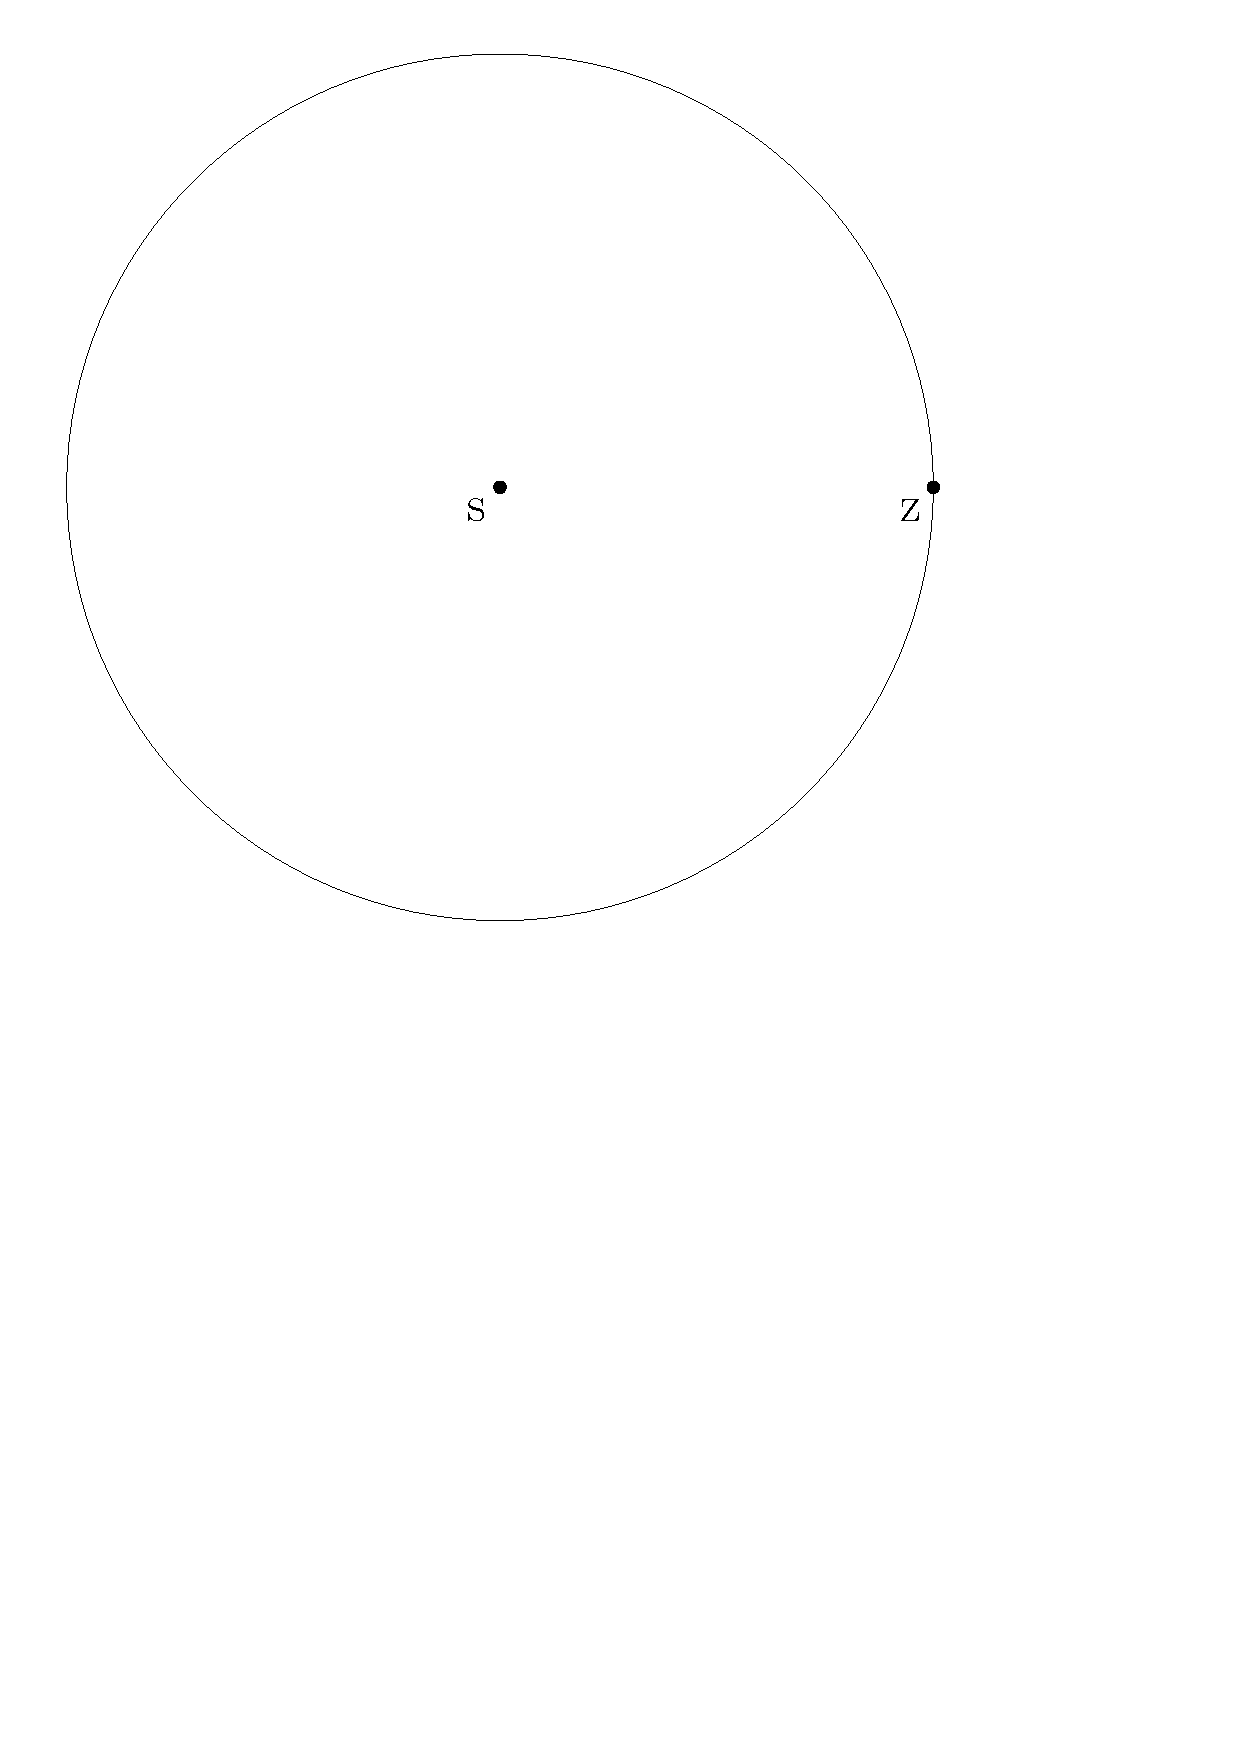
\includegraphics[width = \textwidth]{../media/normaldijkstra.pdf} \\
\caption{Early Stopping}
\label{fig:normalD}
\end{subfigure}
\begin{subfigure}{0.30\textwidth}
\centering
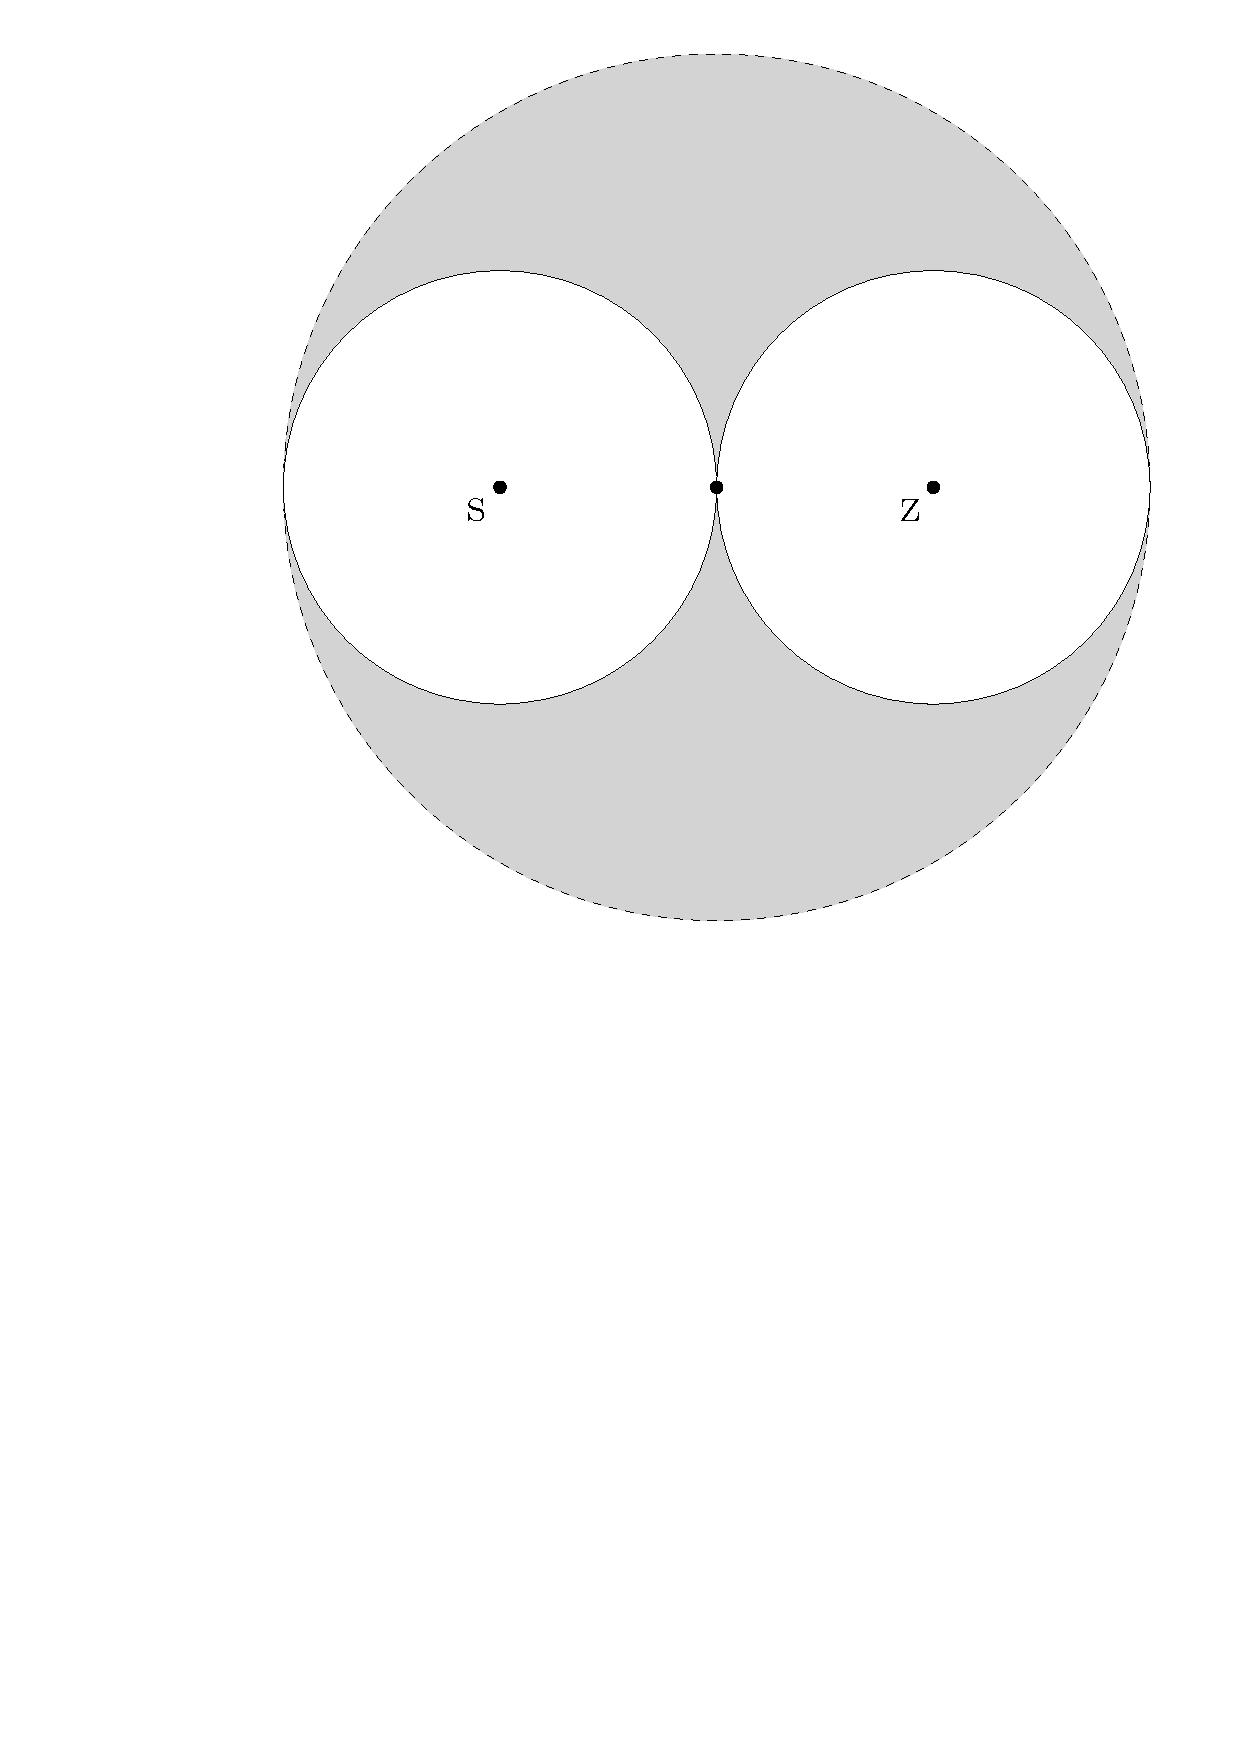
\includegraphics[width = \textwidth]{../media/bidijkstra.pdf} \\
\caption{Bidirectional Dijkstra}
\label{fig:biD}
\end{subfigure}
\begin{subfigure}{0.30\textwidth}
\centering
\vspace{1.1cm}
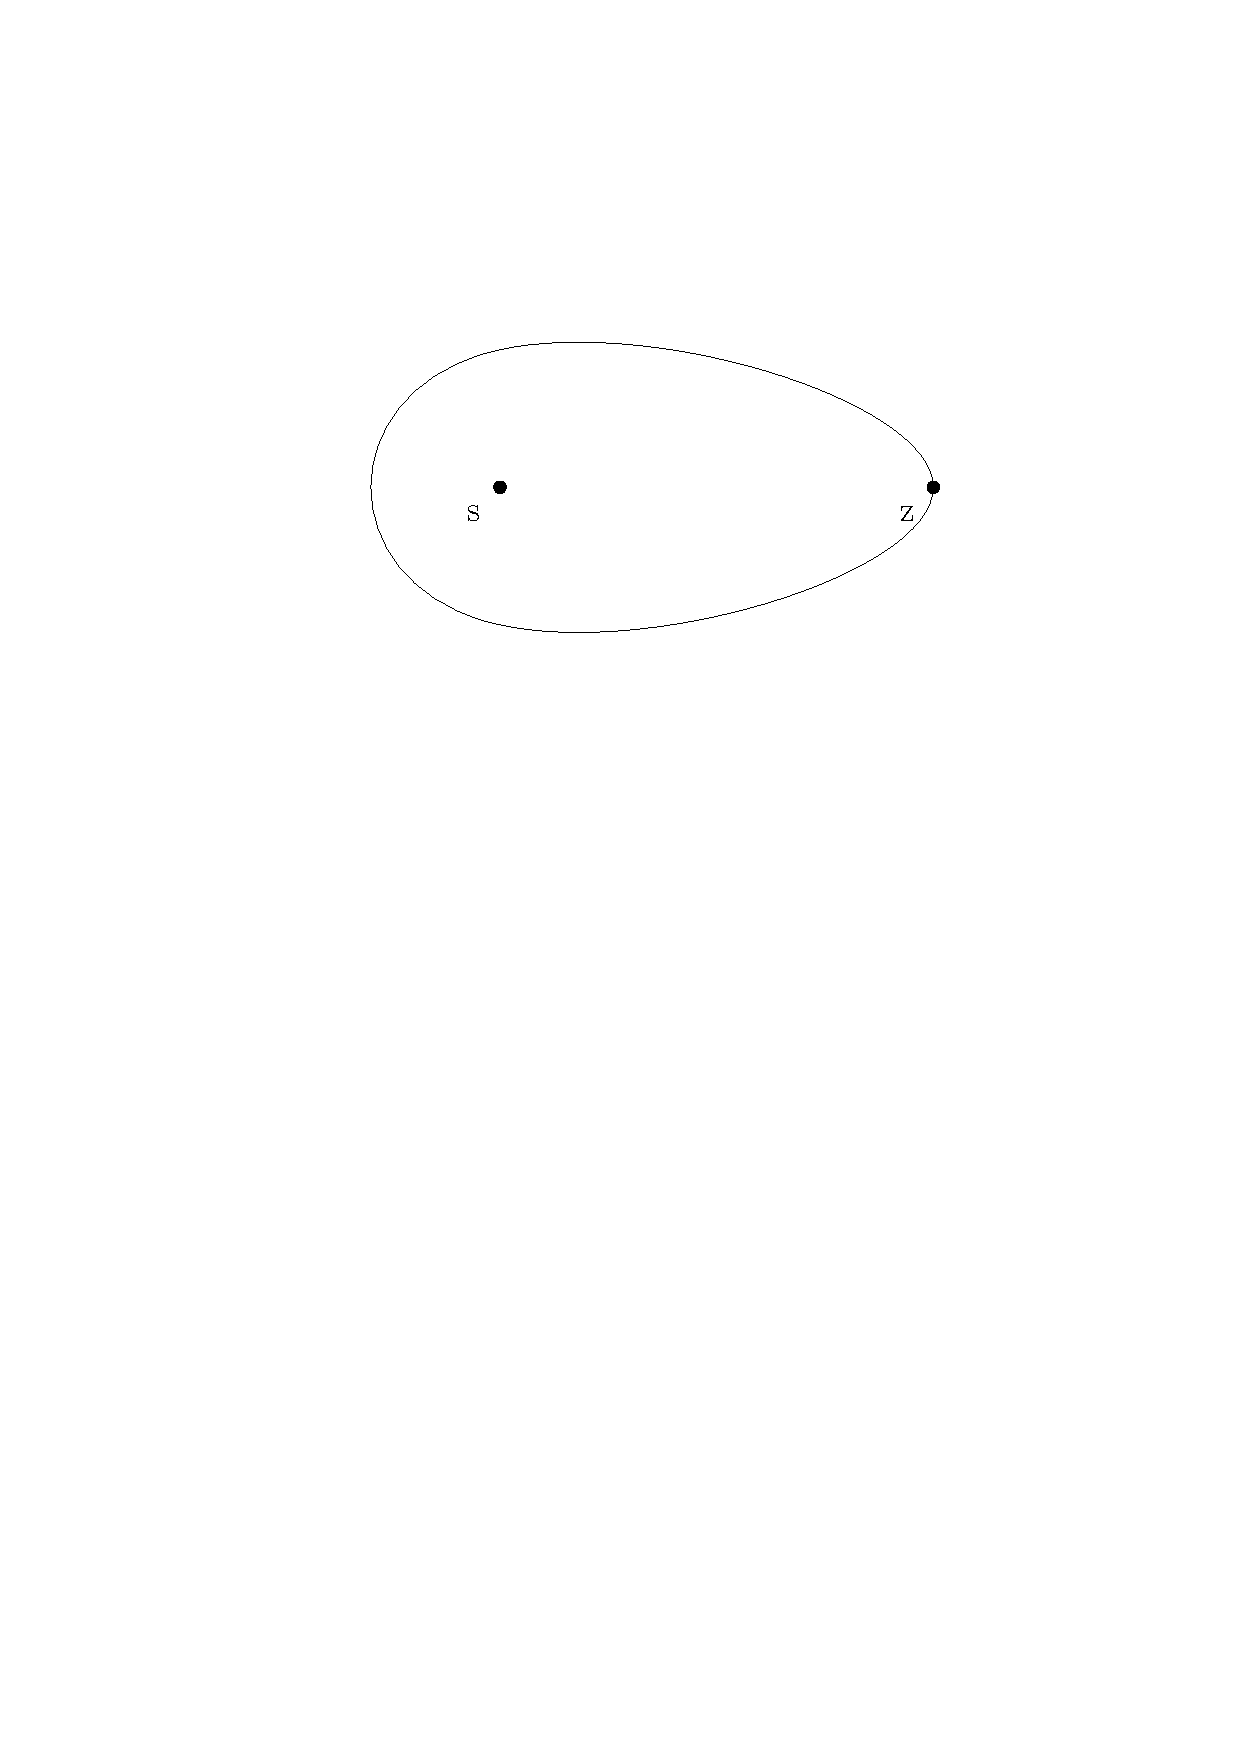
\includegraphics[width = \textwidth]{../media/stardijkstra.pdf} \\
\vspace{0.9cm}
\caption{A*-Algorithmus}
\label{fig:starD}
\end{subfigure}
\caption[Speed-up Techniken für den Dijkstra Algorithmus]
{\centering Speed-up Techniken für den Dijkstra Algorithmus 
\par\justifying\scriptsize
Zu sehen sind unterschiedliche Möglichkeiten den Dijkstra Algorithmus zu beschleunigen.
Der normal für den kompletten Graphen ausgeführte Dijkstra kann nach erreichen des Zielpunktes angehalten werden (a).
Es können parallel zwei Dijkstras jeweils auf Start- und Zielpunkt ausgeführt werden (b).
Der theortisch eingesparte Bereich, gegenüber dem \textit{Early Stopping} ist grau eingefärbt.
Die Auswahl der betrachteten Ecken kann in Richtung des Zielpunktes gelenkt werden (c), wodurch im Gegensatz zur standardmäßig kreisförmigen Ausbreitung weniger Ecken betrachtet werden müssen.
}
\label{speedup}
\end{figure}

\paragraph*{A*:}
Der $A*~$Algorithmus ist eine Variante des Dijkstras, die den Suchraum in Richtung der Zielecke lenkt.
Es wird durch eine Funktion für jede Ecke die Distanz zum Ziel geschätzt.
Diese wird mit den Kantengewichten verrechnet, damit Ecken in Zielrichtung früher markiert werden.
Die standardmäßig kreisförmige Ausbreitung des Dijkstras wird mit dem A* zu einem Oval gestreckt.
Da der Zielpunkt so früher erreicht wird, müssen weniger Iterationen durchgeführt werden.

Diese und weitere Möglichkeiten sind in \cite[209--213]{kurt} ausführlich beschrieben.

\newpage
\subsection{Isochronen Berechnung}

Isochronen sind Linien gleicher Zeit (griech.: \textit{iso} = gleich + \textit{chronos} = Zeit).

Wenn in einem gewichteten Graphen die Kanten die benötigte Zeit enthalten um von einer Ecke zur nächsten zu gelangen, können damit Analysen zur Erreichbarkeit durchgeführt werden.
Dazu wird ein \gls{ssp} für eine zentrale Ecke~$z$ mit einem gegebenen Zeitlimit~$t$ gelöst.
Isochronen können mit unterschiedlichen Methoden berechnet werden.
Das resultierende Objekt ist immer ein Polygon, welches jeden in gegebenem Zeitlimit erreichbaren Punkt beinhaltet.


\subsubsection{Gitterbasierter Ansatz}

Beim \textit{Marching Squares} Algorithmus wird um das Zentrum ein Gitter über dem Graphen gebildet~(Abb.~\ref{fig:grid1}).
Die Eckpunkte des Gitters erhalten dabei die Werte des nächsten Punktes auf dem Graphen(Abb.~\ref{fig:grid2}).
Anschließend werden auf den Kanten des Gitters diejenigen Punkte markiert, bei denen der Wert mit dem gesuchten Zeitlimit übereinstimmt.
In Abbildung~\ref{fig:grid3} wurde das für die Werte $t=5$ und $t=10$ durchgeführt.
Die markierten Punkte werden verbunden und bilden schließlich die Isochrone.

Der Vorteil dieses Algorithmus ist, dass die Maschengröße des Gitters angepasst werden kann.
Bei sehr kleinen Maschen liefert der Algorithmus ein sehr genaues Ergebnis.
Allerdings werden dabei mehr Ressourcen zur Berechnung benötigt.
Daher sollten lediglich kleine Gebiete sowie geringe Zeitlimits berechnet werden.
Bei weiten Maschen ist der Algorithmus dagegen sehr schnell und kann größere Distanzen und längere Zeitspannen berechnen.
Das Ergebnis ist jedoch dementsprechend ungenauer.
In Abbildung~\ref{fig:grid4} wurde die Größe der Maschen beispielsweise ungeschickt gewählt, da eine Ecke mit Abstand vier Minuten vom Zentrum liegt und dadurch außerhalb der fünf-Minuten-Isochrone.

\begin{figure}[htb]
\centering
\begin{subfigure}{0.47\textwidth}
\centering
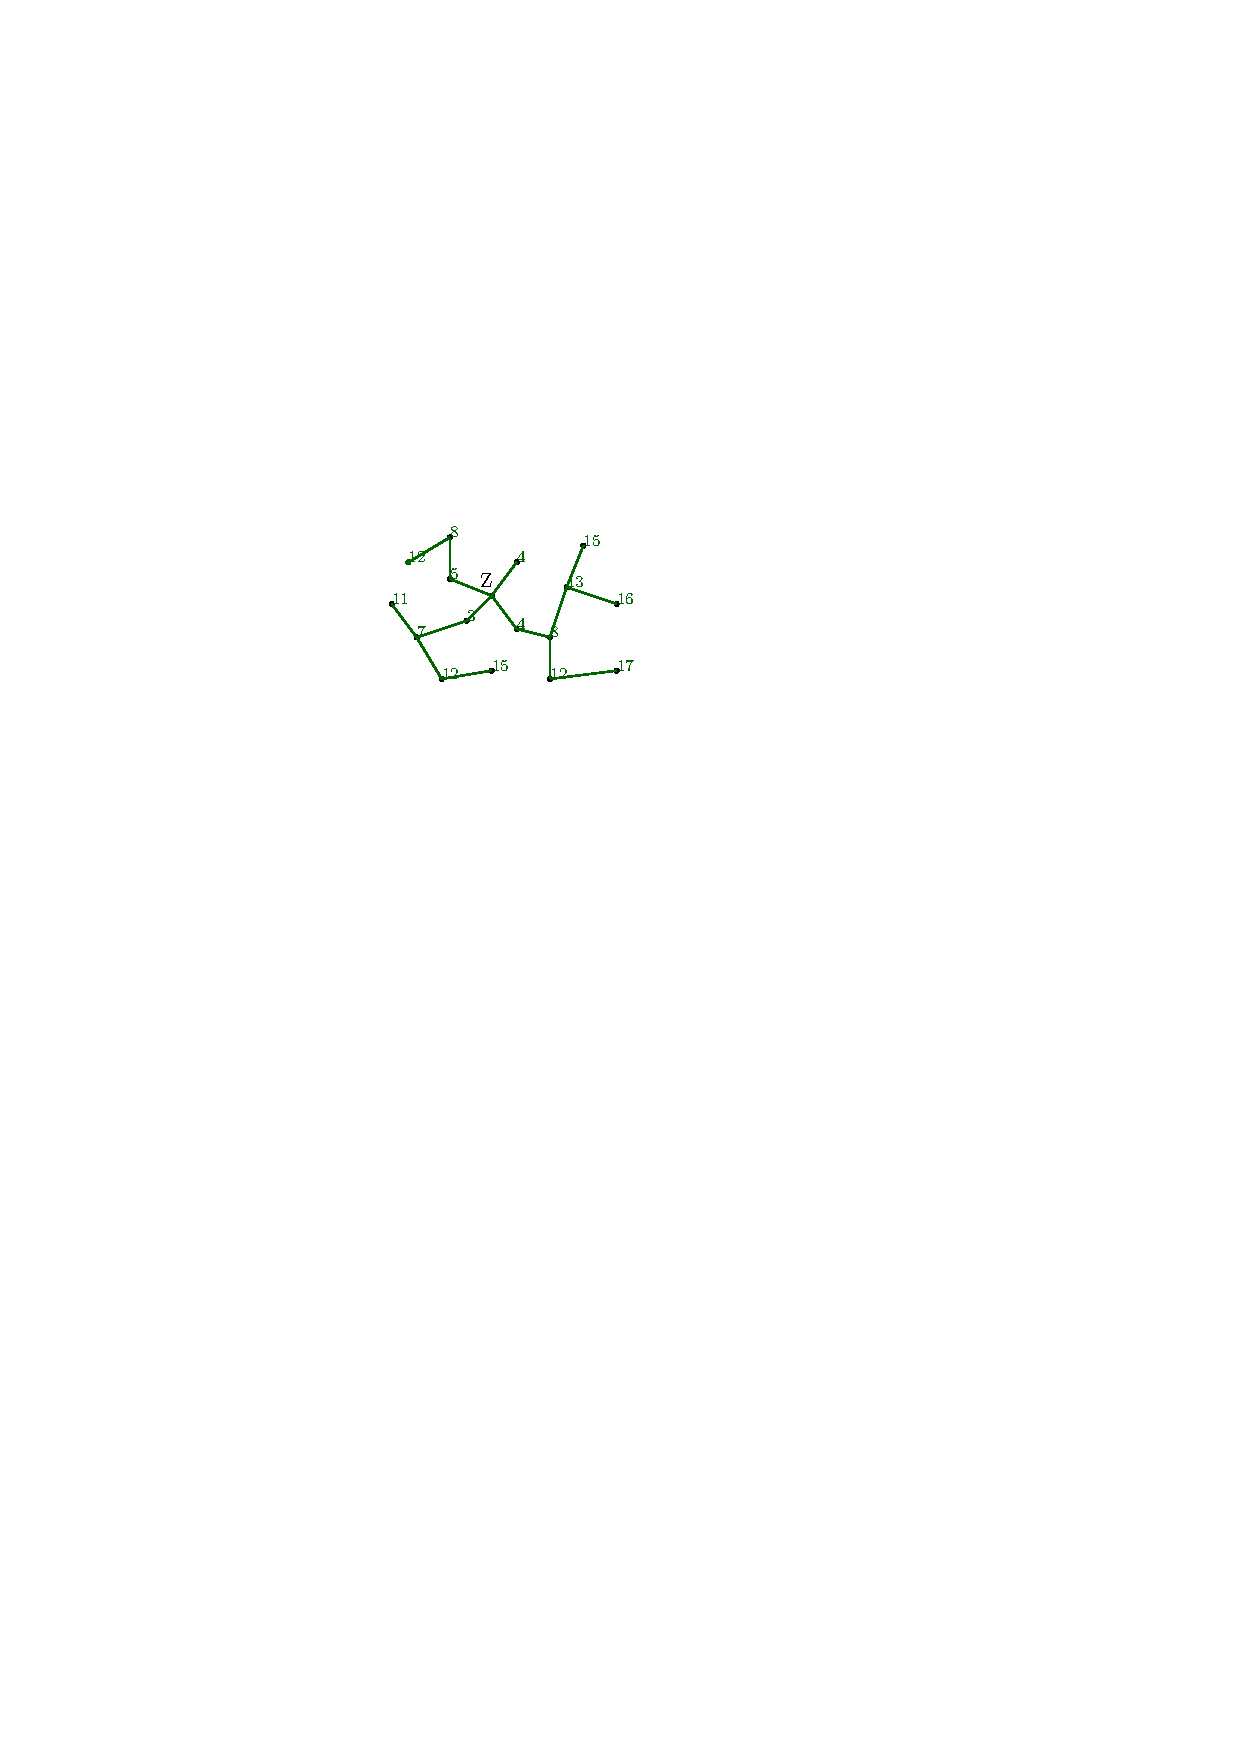
\includegraphics[width = \textwidth]{../media/grid.pdf} \\
\caption{Basis Graph mit kürzesten Wegen}
\vspace{0.3cm}
\label{fig:grid1}
\end{subfigure}
\begin{subfigure}{0.47\textwidth}
\centering
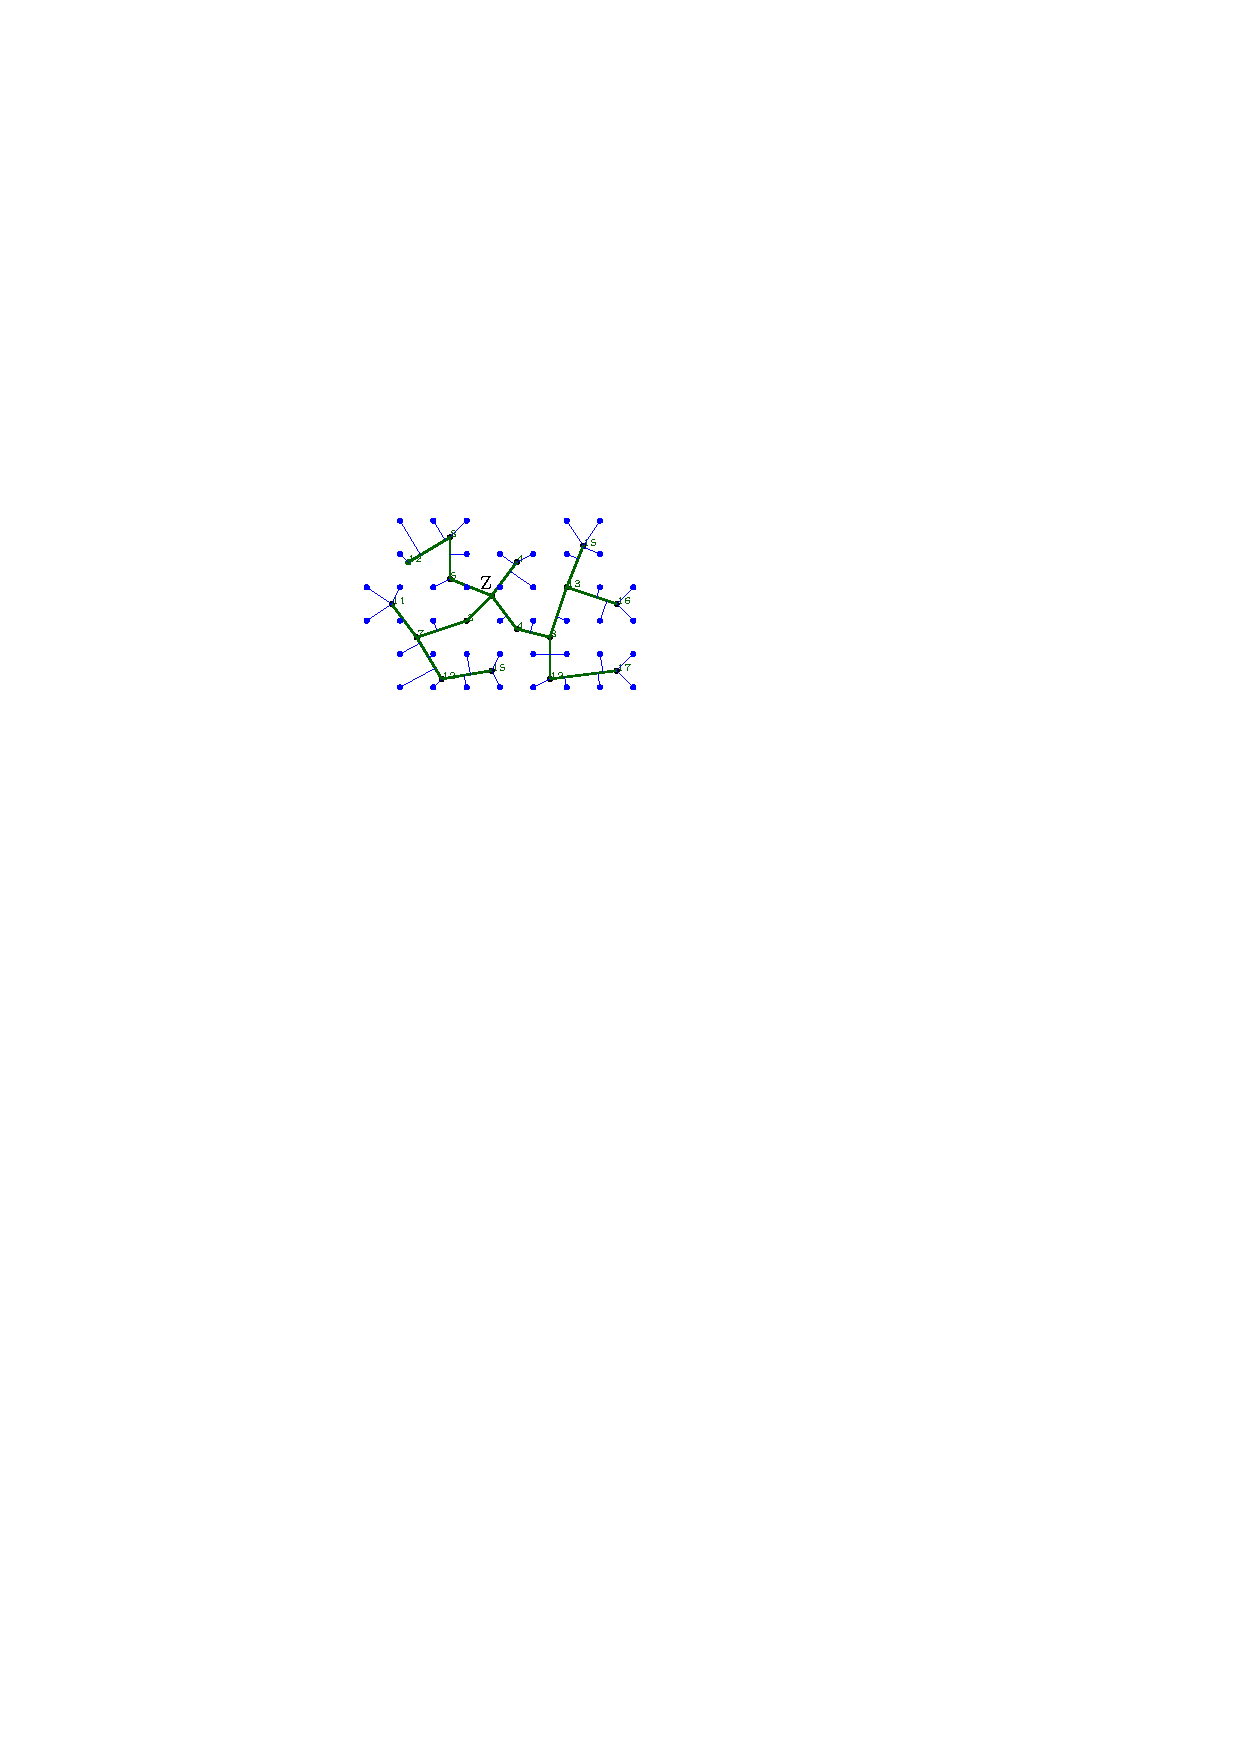
\includegraphics[width = \textwidth]{../media/gridsnap.pdf} \\
\caption{Gitterbildung}
\vspace{0.3cm}
\label{fig:grid2}
\end{subfigure}
\begin{subfigure}{0.44\textwidth}
\centering
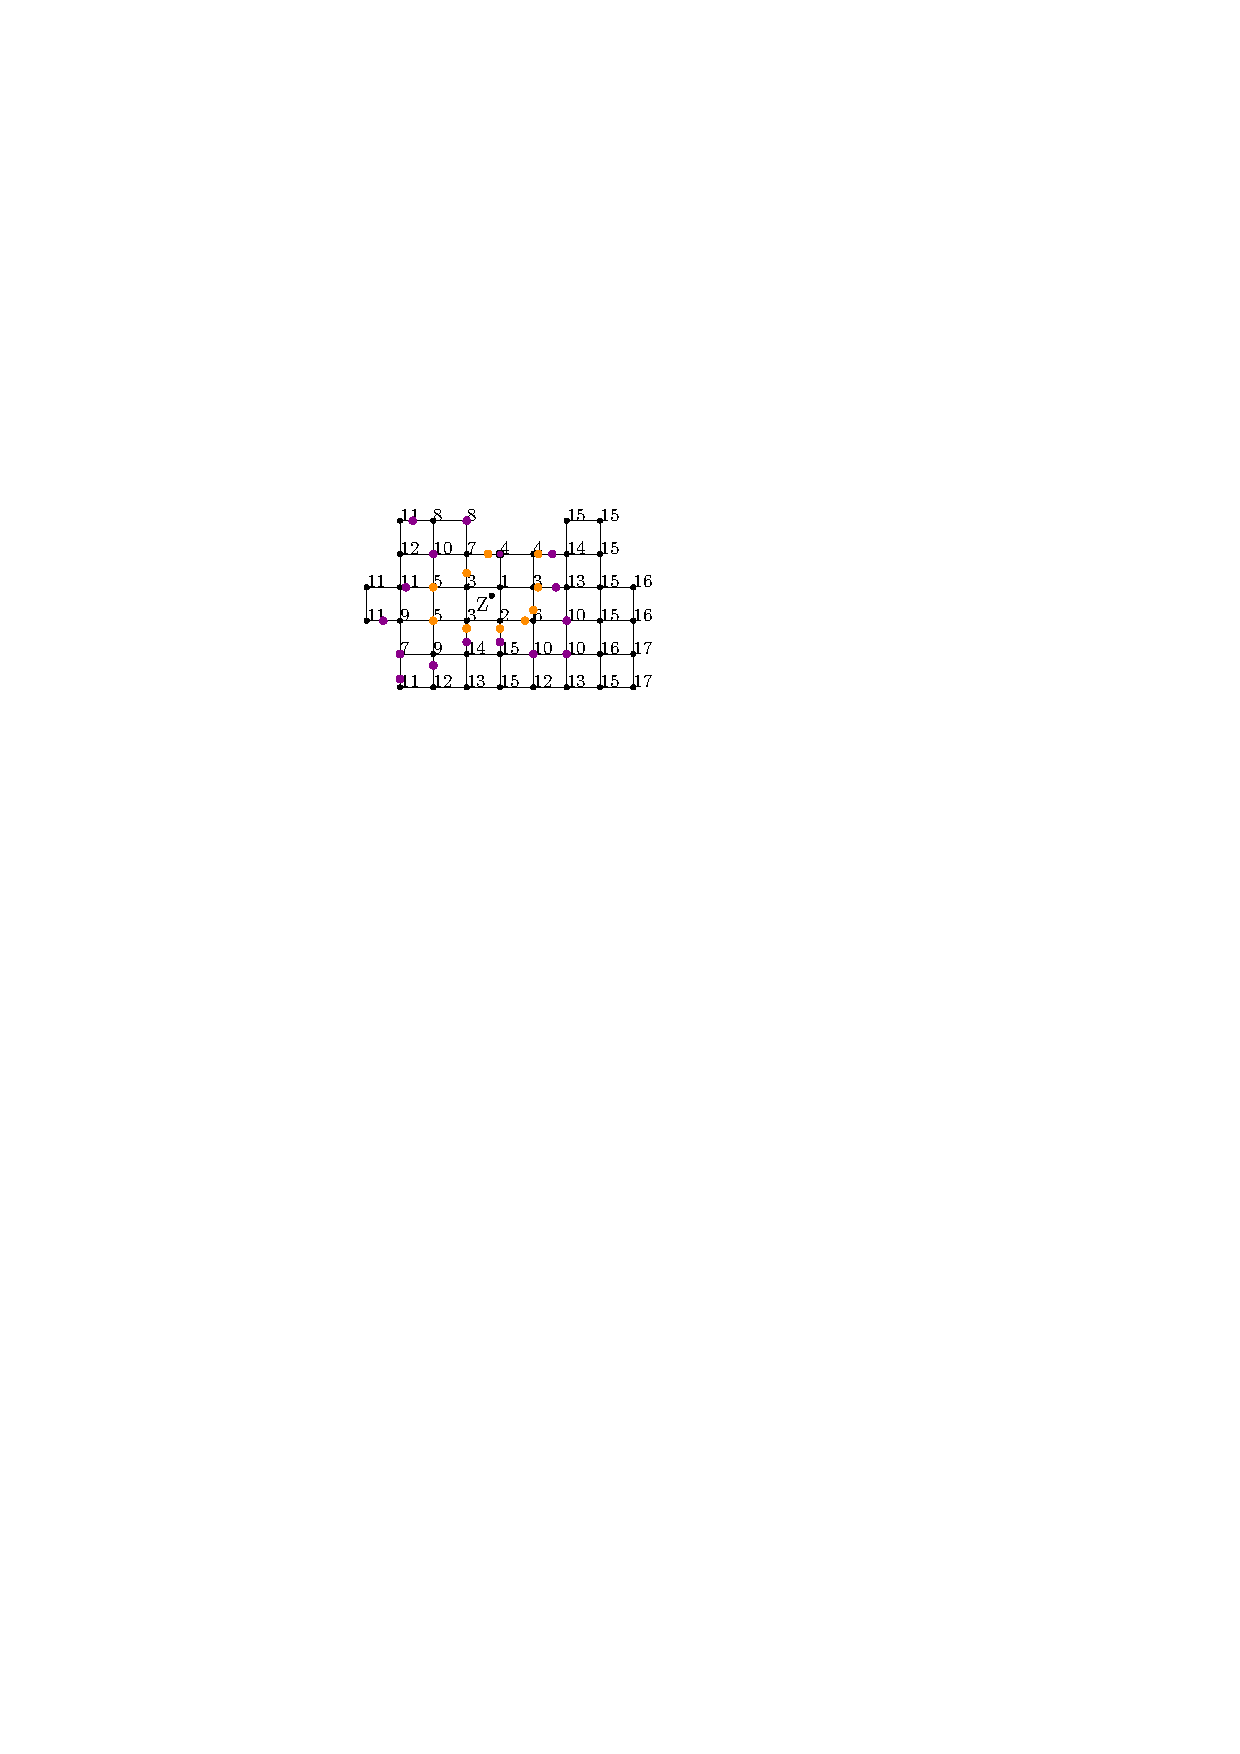
\includegraphics[width = \textwidth]{../media/gridedge.pdf} \\
\caption{Kantenmarkierung}
\label{fig:grid3}
\end{subfigure}
\begin{subfigure}{0.47\textwidth}
\centering
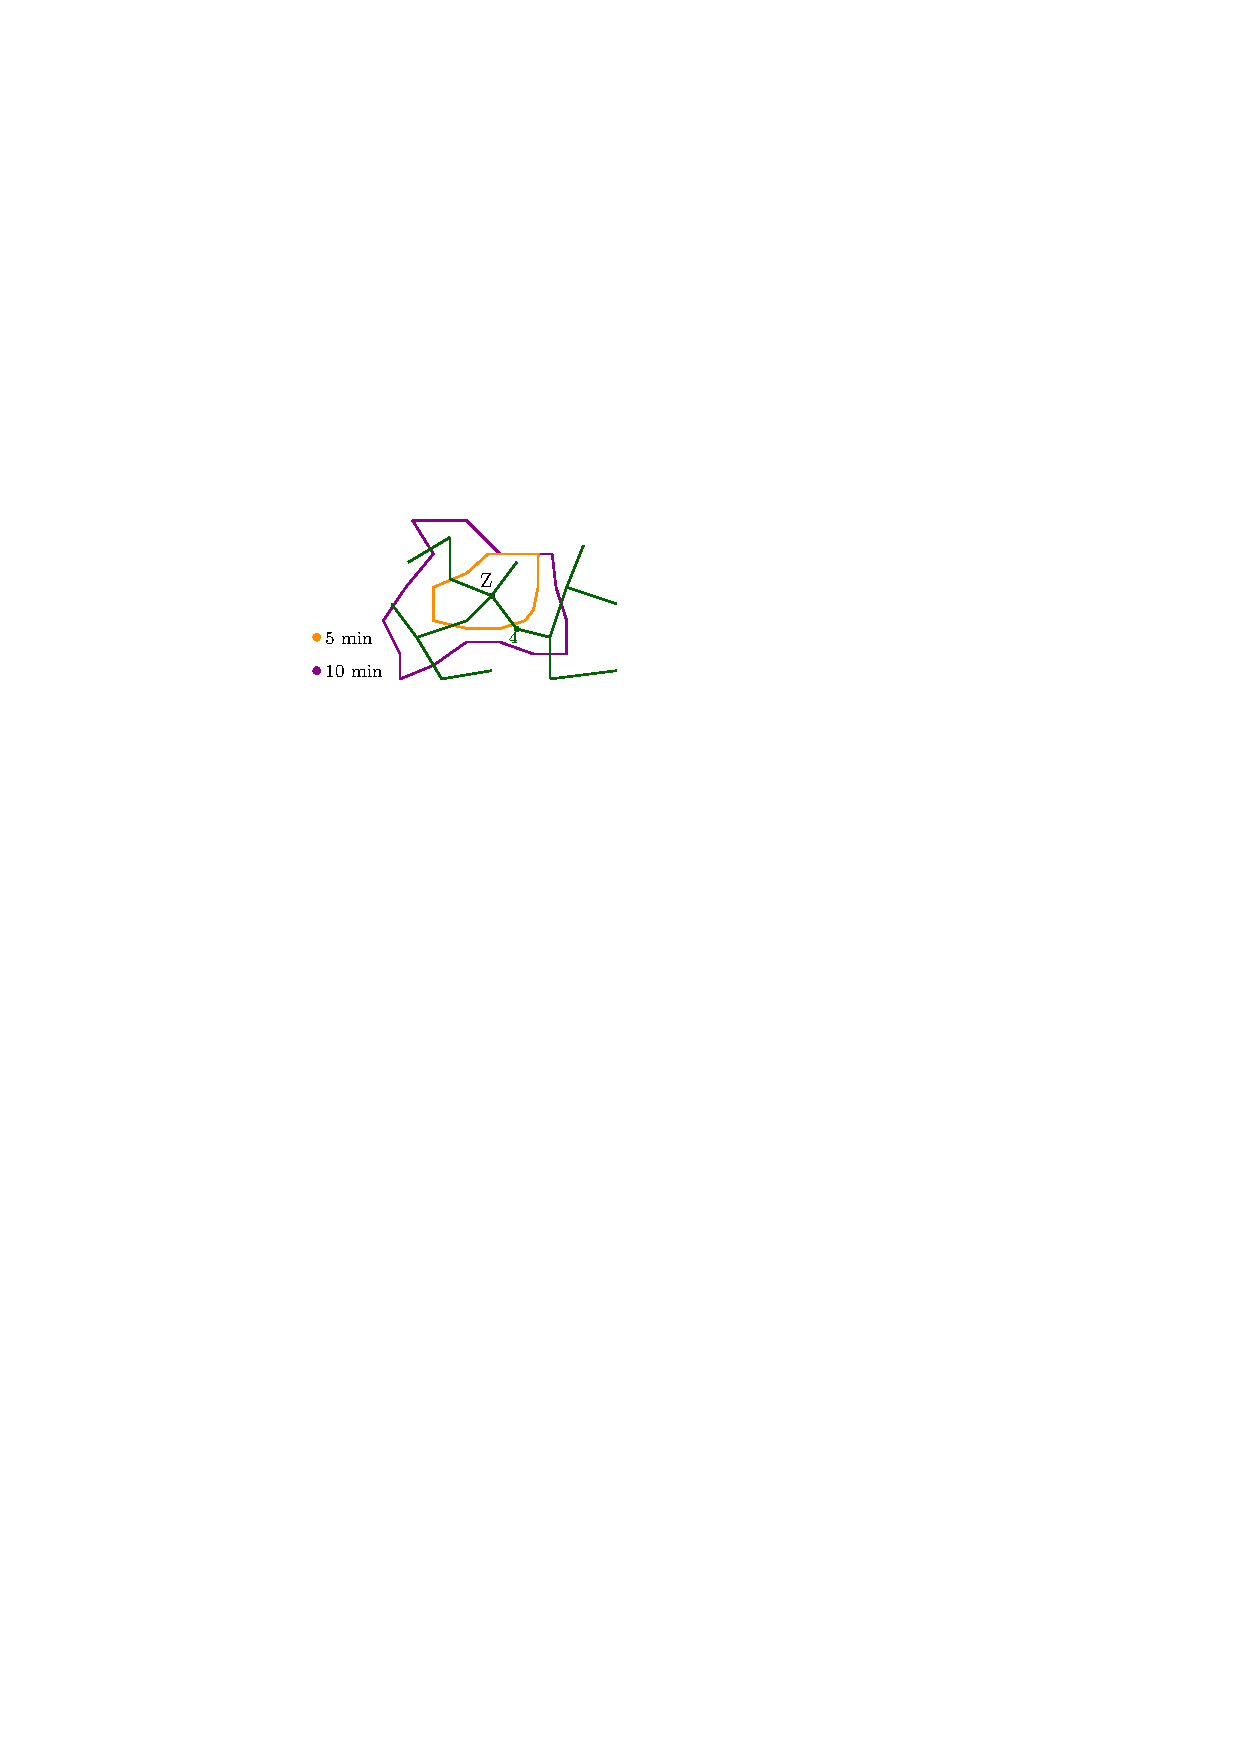
\includegraphics[width = \textwidth]{../media/gridiso.pdf} \\
\caption{Resultierende Isochrone}
\label{fig:grid4}
\end{subfigure}
\caption[Funktionsweise des Marching Squares Algorithmus]
{\centering Funktionsweise Marching Squares Algorithmus
\par\justifying\scriptsize
Über einem Graphen mit von Punkt $Z$ aus benötigten Zeiten als Wert jeder Ecke (a) wird ein Gitter platziert.
Die Eckpunkte dieses Gitters sind in (b) als blaue Punkte dargestellt.
Ihnen werden die Wert des Punktes auf dem Graphen zugeteilt, zu dem sie den geringsten Abstand haben (c).
Die gesuchte Zeit wird auf den Kanten des Gitters markiert (c).
Die Punkte werden zu Polygonen verbunden und als Isochrone über dem Graphen dargestellt (s).
}
\label{grid}
\end{figure}

\subsubsection{Dreiecksvermaschung}
\cite{isochrones} beschreiben eine anschauliche Methode, um Isochronen zu berechnen.
Nach der Lösung des \gls{ssp}s werden den Ecken des Graphen die geographische Koordinate der repräsentierten Kreuzung zugeteilt.
Die Kanten werden nicht benötigt und daher entfernt.
Es liegt demnach eine 3D-Punktwolke vor.
Jeder Ecke wird nun die benötigte Zeit zugewiesen, mit der diese zu erreichen ist.
Anschließend werden die Ecken nach dem Delaunay Triangulationsverfahren vermascht.
Dadurch entsteht eine Art Trichter, mit der Startecke als Tiefpunkt auf der Höhe Null.
Wird dieser Trichter auf Höhe des Zeitlimits geschnitten, entsprechen von oben betrachtet die Randkanten des Trichters der Isochrone.


\subsubsection{Formenbasierter Ansatz}
\label{sec:form}
Die Implementierung des \gls{ors} zur Berechnung von Isochronen verwendet einen Form-basierten Ansatz.
Zuerst werden mit dem in Kapitel ~\ref{sec:dijkstra} bereits ausführlich erklärten Dijkstra Algorithmus alle in gegebener Zeit erreichbaren Kanten markiert.
Anschließend werden die geographischen Punkte (Pillar Nodes) aus der $WayGeometry$ der Kante extrahiert (Siehe Kapitel ~\ref{sec:osmgraph} auf Seite ~\pageref{sec:osmgraph}).
Um jeden der extrahierten Punkte wird ein kreisförmiger Pufferbereich gelegt.
Dadurch können nahe beieinanderliegende Punkte übersprungen werden.
Mit den verbleibenden Punkten wird eine Punktwolke generiert.
Auf dieser Punktwolke wird nun der Alpha-Shape Algorithmus (\cite{akkiraju1995alpha}) angewandt, um die Isochrone als Hülle um die erreichbaren Wegsegmente zu zeichnen.
Dieser Ansatz liefert präzise Ergebnisse bei schnellen Berechnungszeiten.
Die Verwendung der Alpha-Shapes verhindert allerdings die Möglichkeit der Darstellung von nicht erreichbaren Gebieten innerhalb der Isochronen.
